\documentclass[11pt]{article}

% --- packages -----------------------------------------------------------------
\usepackage[a4paper, margin=1in]{geometry}
\usepackage{amsmath, amssymb, amsthm, mathtools}
\usepackage{graphicx}
\usepackage{booktabs}
\usepackage{microtype}
\usepackage{xcolor}
\usepackage[most]{tcolorbox}
\usepackage{enumitem}
\usepackage{caption}
\usepackage{tikz}
\usetikzlibrary{arrows.meta, positioning, fit, backgrounds, calc}
\usepackage[numbers, sort&compress]{natbib}
\usepackage{hyperref}

\hypersetup{colorlinks=true, linkcolor=black!60!blue,
  citecolor=black!60!blue, urlcolor=black!50!blue}

\sloppy \hbadness=4000 \emergencystretch=3em

% --- theorem environments -----------------------------------------------------
\newtheorem{proposition}{Proposition}
\newtheorem{theorem}[proposition]{Theorem}
\newtheorem{corollary}[proposition]{Corollary}
\newtheorem{lemma}[proposition]{Lemma}
\theoremstyle{definition}
\newtheorem{remark}{Remark}

% --- colours and boxes --------------------------------------------------------
\definecolor{derivframe}{HTML}{1a3a5c}\definecolor{derivblue}{HTML}{e8f0f8}
\definecolor{bayesframe}{HTML}{8a6d2e}\definecolor{bayesbg}{HTML}{f6efe2}
\definecolor{intuiframe}{HTML}{2f6b34}\definecolor{intuibg}{HTML}{e9f1e3}
\definecolor{auditframe}{HTML}{6b2356}\definecolor{auditbg}{HTML}{f1e6ee}
\definecolor{accent}{HTML}{b5341a}

\newtcolorbox{derivation}[1][]{enhanced, breakable, colback=derivblue,
  colframe=derivframe, boxrule=0.6pt, arc=2pt, fonttitle=\bfseries,
  coltitle=white, colbacktitle=derivframe,
  attach boxed title to top left={xshift=4pt, yshift=-2pt},
  boxed title style={arc=2pt, boxrule=0pt}, title={\small Derivation #1},
  left=8pt, right=8pt, top=14pt, bottom=8pt}
\newtcolorbox{bayesianview}[1][]{enhanced, breakable, colback=bayesbg,
  colframe=bayesframe, boxrule=0.6pt, arc=2pt, fonttitle=\bfseries,
  coltitle=white, colbacktitle=bayesframe,
  attach boxed title to top left={xshift=4pt, yshift=-2pt},
  boxed title style={arc=2pt, boxrule=0pt}, title={\small Bayesian view #1},
  left=8pt, right=8pt, top=14pt, bottom=8pt}
\newtcolorbox{intuition}[1][]{enhanced, breakable, colback=intuibg,
  colframe=intuiframe, boxrule=0.6pt, arc=2pt, fonttitle=\bfseries,
  coltitle=white, colbacktitle=intuiframe,
  attach boxed title to top left={xshift=4pt, yshift=-2pt},
  boxed title style={arc=2pt, boxrule=0pt}, title={\small Reading #1},
  left=8pt, right=8pt, top=14pt, bottom=8pt}
\newtcolorbox{auditbox}[1][]{enhanced, breakable, colback=auditbg,
  colframe=auditframe, boxrule=0.6pt, arc=2pt, fonttitle=\bfseries,
  coltitle=white, colbacktitle=auditframe,
  attach boxed title to top left={xshift=4pt, yshift=-2pt},
  boxed title style={arc=2pt, boxrule=0pt}, title={\small Numerical check #1},
  left=8pt, right=8pt, top=14pt, bottom=8pt}

% --- macros -------------------------------------------------------------------
\newcommand{\R}{\mathbb{R}}
\newcommand{\N}{\mathcal{N}}
\newcommand{\E}{\mathbb{E}}
\newcommand{\Sig}{\Sigma}
\newcommand{\Dt}{\Delta_t}
\newcommand{\Qt}{Q_t}
\newcommand{\given}{\,|\,}
\newcommand{\dd}{\mathrm{d}}
\newcommand{\T}{^{\!\top}}
\newcommand{\Jd}{J_{\mathrm d}}
\DeclareMathOperator{\Cov}{Cov}
\DeclareMathOperator{\Var}{Var}
\DeclareMathOperator{\diag}{diag}

% --- tikz styles for factor graphs --------------------------------------------
\tikzset{
  var/.style={circle, draw=derivframe, fill=white, line width=0.8pt,
              minimum size=8mm, inner sep=0pt},
  fac/.style={rectangle, draw=derivframe, fill=derivframe!18, line width=0.8pt,
              minimum size=5mm, inner sep=2pt},
  obs/.style={rectangle, draw=accent, fill=accent!15, line width=0.8pt,
              minimum size=5mm, inner sep=2pt},
  edge/.style={line width=0.8pt, derivframe!70},
  fwd/.style={-{Stealth[length=3mm]}, line width=1.3pt, accent},
  bwd/.style={-{Stealth[length=3mm]}, line width=1.3pt, intuiframe},
}

\title{\bfseries Gaussian Belief Propagation for the Diffusion Score\\[2pt]
\large The fully solvable AR(1)$+$OU chain: joint score, factor graph,
sum--product,\\ \large Kalman, closed-form bulk analysis, and the breakdown of AMP}
\author{Giovanni Mantovani\\[2pt]
\small Bocconi University, MSc Data Science\\[1pt]
\small supervised by M.\ M\'ezard and J.\ Garnier-Brun}
\date{\today}

\begin{document}
\maketitle

\begin{abstract}
\noindent
We study the \emph{joint} score of a diffusion model on a sequence of
correlated frames in the only setting where everything can be carried to the
end in closed form: a stationary Gaussian \textsc{ar}(1) Markov chain whose
frames are independently corrupted by a variance-preserving
Ornstein--Uhlenbeck channel. The note is written to be self-contained: we
derive the forward channel from the OU stochastic differential equation, prove
the three Gaussian lemmas used by every later computation, derive the clean
joint law and its tridiagonal precision, the noised law
$P_t(x)=\N(0,\Sig_t)$, and the joint score $S(x,t)=-\Sig_t^{-1}x$ both
directly and through Tweedie's identity, whose proof we give in full together
with its denoiser, expected-noise, and tilted-measure readings and the
reverse-time SDE in which the score is the drift. The $K=2$ case is worked out
completely as the smallest example of inter-frame coupling. We then write the
posterior $p(a\given x)$ as a factor graph (a caterpillar tree), prove it is a
tree, derive belief propagation from scratch with an explicit bookkeeping
convention that avoids the double-counting trap, execute every message by hand
on the $K=3$ chain --- symbolically and numerically --- and identify the
sweeps with the Kalman filter and RTS smoother. Gaussianity of all messages is
an \emph{exact algebraic closure}, not a central limit effect. New to this
version, we solve the chain in closed form in its homogeneous bulk: the exact
posterior covariance is geometric, $(J^{-1})_{i,i+d}=q^{\,d}/\sqrt{\Jd^2-4\beta^2}$,
the BP message precision has the explicit fixed point
$\lambda^\ast=(\Jd+\sqrt{\Jd^2-4\beta^2})/2$ which exists for \emph{every}
coupling, and the AMP/TAP variance closure has the explicit fixed point
$V=(\Jd-\sqrt{\Jd^2-8\beta^2})/4\beta^2$ which exists \emph{iff}
$\Jd\ge2\sqrt2\,|\beta|$ --- giving an exact breakdown time $t_c(\alpha)$ and a
critical coupling $\alpha_c=\sqrt2-1$ below which AMP never breaks down. BP,
AMP, and mean field share the same posterior mean, hence the \emph{same
score}; they differ only in the variance, where AMP first deviates at fourth
order in the coupling, $V_{\textsc{amp}}-V_{\mathrm{exact}}=2\beta^4/\Jd^5+\dots$,
and then ceases to exist --- making quantitative J.~Garnier-Brun's remark that
a central limit theorem ``on two points'' need not hold. Two experiments
close the note: the locality of the score (the truncation error of a radius-$r$
estimator decays exactly as $q^{\,r}$), and the lifecycle of the precision
matrix $\Sig_t^{-1}$ along diffusion time, including the corrected band-fill
law $(Q_t)_{i,i+d}=(-1)^{d-1}(2t)^{d-1}(Q_0^d)_{i,i+d}+O(t^d)$ (no
$1/(d-1)!$ factor). Every quantitative claim is verified by an independent
numerical audit (\textbf{72/72 checks pass}); three executed companion
notebooks reproduce every number and figure.
\end{abstract}

\tableofcontents
\medskip
\hrule
\medskip

% =============================================================================
\section{Introduction and motivation}\label{sec:intro}
% =============================================================================

\paragraph{What generative diffusion is.}
Generative diffusion aims at producing artificial data $a\in\R^d$ distributed
according to a law $P_0(a)$ that is not known explicitly but from which we
hold $n$ examples. The recipe has two halves: \emph{noising} the data by a
diffusion process until all structure is destroyed, then \emph{denoising} by a
reverse-time diffusion whose drift contains a trained vector field --- the
\emph{score} $\nabla_x\log P_t(x)$
\citep{mezard2025generative,song2021scorebased,vincent2011connection}. This is
the state of the art in image and video generation, and the same trained score
also gives likelihood estimates of new data points.

\paragraph{Our setting: dynamic objects.}
This project studies diffusion on \emph{dynamic objects}: ordered sequences
with an internal time, the canonical example being a short video clip. A
dynamic object is a sequence of $K$ frames $a_0,\dots,a_{K-1}$, drawn from a
clean joint distribution with \emph{Markov} structure,
\begin{equation}\label{eq:chain-prior}
  P_0(a_0,\dots,a_{K-1})=p_0(a_0)\prod_{u=0}^{K-2}M(a_{u+1}\given a_u),
\end{equation}
and the diffusion paradigm corrupts each frame independently with an
Ornstein--Uhlenbeck (OU) process at diffusion time $t$. Sampling from $P_0$
then requires the \emph{joint score field}
\begin{equation}\label{eq:joint-score-def}
  S(x,t):=\nabla_x\log P_t(x_0,\dots,x_{K-1})\in\R^{K}.
\end{equation}

\begin{remark}[Joint, not marginal --- the central correction]\label{rmk:joint}
The object of interest is the score of the \emph{joint} law of the whole
sequence. It is emphatically \emph{not} the per-frame marginal score
$\nabla_{x_k}\log p_t(x_k)$, which integrates out every other frame and would
be the right object only if the frames were generated independently. A video
is \emph{one} sample of a joint law, not $K$ samples of a marginal; the joint
score couples each frame to the entire trajectory through the full posterior
$P(a\given x)$. Every formula below is a joint-score formula. (For the
model of this note the per-frame marginal score is the trivial $-x_k$ at every
$t$ --- see \S\ref{sec:K2} --- so the marginal formulation would erase
precisely the structure we want to study.)
\end{remark}

\paragraph{Why the Gaussian \textsc{ar}(1) chain.}
We take the simplest nontrivial instance of \eqref{eq:chain-prior}: a
stationary Gaussian \textsc{ar}(1) chain of scalar frames. Three reasons make
it the right testbed.
\begin{enumerate}[leftmargin=1.6em, itemsep=1pt]
\item \textbf{Everything is closed form.} The clean law, the noised law, the
posterior, the score, the message-passing fixed points, even the breakdown
boundary of AMP --- all are explicit formulas, each verified independently.
\item \textbf{It separates the two structural mechanisms.} Gaussianity is
responsible for the \emph{linearity} of the score; Markovianity is responsible
for the \emph{tridiagonal sparsity} of the clean precision. The literature
often conflates them; here each can be traced separately.
\item \textbf{It is the cleanest stage for the algorithmic question.} The
posterior is a tree-structured graphical model, so belief propagation (BP) is
exact and $O(K)$; the same model viewed as a Gaussian Markov random field lets
us run the AMP/TAP closure side by side and see precisely where, and why, the
dense-graph approximation fails on a chain.
\end{enumerate}

\paragraph{Questions this note answers.}
The note grew out of working sessions with M.~M\'ezard and J.~Garnier-Brun and
is organised around their questions:
\begin{itemize}[leftmargin=1.6em, itemsep=1pt]
\item Derive the clean joint, the noised joint, and the score --- both directly
and ``the Bayesian way'' (Tweedie). Do the two agree? (\S\ref{sec:noisy}: yes,
identically; audited.)
\item Write the posterior, draw its factor graph, run BP. Are the messages
Gaussian? Is the posterior Gaussian? Is BP exact here? (\S\ref{sec:bpK}: yes,
yes, yes --- by algebraic closure and tree-exactness, \emph{not} by any central
limit argument.)
\item Apply AMP. Is AMP the same as BP here? (\S\ref{sec:amp}: the \emph{score}
is the same --- the mean solves the same linear system --- but the variance
closures differ, and AMP's has no fixed point beyond an explicit boundary.)
\item What is the difference between running strictly local messages and the
full forward--backward sweeps? (\S\ref{sec:expA}: the truncation error decays
exactly as $q^{\,r}$ with an explicit $q(\alpha,t)$.)
\item How does the tridiagonal structure of the precision die and come back
along diffusion time? (\S\ref{sec:expB}: the band-fill law, the spectral
flow, and the return to the identity, all explicit.)
\end{itemize}

\paragraph{New closed-form results.}
Beyond consolidating the derivations, this version contains five results we
have not seen stated in this form elsewhere (all proved in
\S\ref{sec:bulk}--\S\ref{sec:amp} and verified by the audit):
\begin{enumerate}[leftmargin=1.6em, itemsep=1pt]
\item the exact \emph{bulk posterior covariance} of the chain,
  $(J^{-1})_{i,i+d}=q^{\,d}/\sqrt{\Jd^2-4\beta^2}$, with
  $q=(\Jd-\sqrt{\Jd^2-4\beta^2})/2|\beta|$;
\item the BP message-precision fixed point
  $\lambda^\ast=(\Jd+\sqrt{\Jd^2-4\beta^2})/2$, which exists for \emph{every}
  $(\alpha,t)$ --- BP never breaks down on the chain;
\item the AMP/TAP variance fixed point
  $V=(\Jd-\sqrt{\Jd^2-8\beta^2})/4\beta^2$ and its existence condition
  $\Jd\ge2\sqrt2|\beta|$, hence an exact breakdown time $t_c(\alpha)$ and the
  critical coupling $\alpha_c=\sqrt2-1\approx0.4142$;
\item the weak-coupling law $V_{\textsc{amp}}-V_{\mathrm{exact}}
  =2\beta^4/\Jd^5+O(\beta^6)$: AMP's variance is correct to second order in
  the coupling and first errs --- always upward --- at fourth;
\item the locality law: the RMS truncation error of the radius-$r$ local
  estimator decays exactly as $q^{\,r}$, with the same $q$ as in (i).
\end{enumerate}

\paragraph{Methodological rule.}
Every numbered claim in this note is backed by a named check in
\texttt{code/numerical\_audit.py}. A statement enters the text only if its
check passes; the audit currently passes \textbf{72/72}. We prefer fewer
results that are certainly right over more that are merely plausible.
Appendix~\ref{app:audit} maps claims to checks.

\paragraph{How to read this note.}
Sections \ref{sec:setup}--\ref{sec:toolbox} fix the model and the Gaussian
toolbox. Sections \ref{sec:clean}--\ref{sec:K2} derive the laws and the score,
ending with the fully explicit $K=2$ case. Sections
\ref{sec:posterior}--\ref{sec:bpK} build the factor graph and belief
propagation, with $K=3$ done entirely by hand. Sections
\ref{sec:bulk}--\ref{sec:amp} contain the closed-form bulk analysis and the
BP/AMP comparison. Sections \ref{sec:expA}--\ref{sec:expB} are the two
experiments. Section \ref{sec:summary} collects what is established and what
comes next. Three executed notebooks
(\texttt{01\_model\_and\_score}, \texttt{02\_belief\_propagation},
\texttt{03\_amp\_and\_experiments}) mirror the structure of the note.

% =============================================================================
\section{Setup, notation, and the OU forward channel}\label{sec:setup}
% =============================================================================

\subsection{The model}

A \emph{sequence} is $K$ scalar frames $a=(a_0,\dots,a_{K-1})\in\R^K$, indexed
by the internal (frame) time $k=0,\dots,K-1$. The frames are generated by a
stationary Gaussian \textsc{ar}(1) Markov chain,
\begin{equation}\label{eq:ar1}
  a_{k+1}=\alpha\,a_k+\eta_k,\qquad \eta_k\sim\N(0,\sigma_\eta^2)\ \text{i.i.d.},
  \qquad |\alpha|<1,\qquad a_0\sim\N(0,\sigma_0^2).
\end{equation}
Throughout we use the \emph{stationary, unit-variance} normalisation
\begin{equation}\label{eq:stationary-norm}
  \sigma_\eta^2=1-\alpha^2,\qquad
  \sigma_0^2=\frac{\sigma_\eta^2}{1-\alpha^2}=1,
\end{equation}
so that $\Var(a_k)=1$ for every $k$ (proved in \S\ref{sec:clean}). The scalar
setting $d=1$ loses nothing: every construction below acts per component.

\subsection{The OU channel, derived from its SDE}

Each frame is corrupted \emph{independently} by the variance-preserving OU
process
\begin{equation}\label{eq:ou-sde}
  \dd x=-x\,\dd t+\sqrt2\,\dd W,\qquad x(0)=a_k .
\end{equation}

\begin{proposition}[The forward channel]\label{prop:channel}
At diffusion time $t\ge0$ the solution of \eqref{eq:ou-sde} started at $a_k$
is the affine Gaussian channel
\begin{equation}\label{eq:ou}
  x_k=e^{-t}a_k+\xi_k,\qquad \xi_k\sim\N(0,\Dt),\qquad \Dt:=1-e^{-2t},
\end{equation}
independent across $k$.
\end{proposition}

\begin{derivation}[\ref*{prop:channel}: solving the linear SDE]
Multiply \eqref{eq:ou-sde} by the integrating factor $e^{t}$:
$\dd(e^{t}x)=e^{t}(\dd x+x\,\dd t)=\sqrt2\,e^{t}\dd W$, so
\[
  x(t)=e^{-t}a_k+\sqrt2\int_0^t e^{-(t-s)}\,\dd W_s .
\]
The stochastic integral is Gaussian with mean zero and variance (It\^o
isometry)
\[
  2\int_0^t e^{-2(t-s)}\,\dd s=1-e^{-2t}=\Dt .
\]
Hence $x_k\sim\N(e^{-t}a_k,\Dt)$, and the channels are independent across $k$
because each frame is driven by its own Brownian motion.
\end{derivation}

\begin{intuition}[: variance preservation and the two clocks]
At $t=0$, $x_k=a_k$ (no corruption); as $t\to\infty$, $x_k\to\N(0,1)$ (pure
noise). In between, $\Var(x_k)=e^{-2t}\cdot1+\Dt=1$ \emph{for all} $t$: the
channel trades signal for noise at constant total variance. Two clocks run
through the whole note and must never be confused: the \emph{frame} index $k$
(internal time of the sequence) and the \emph{diffusion} time $t$ (noise
level).
\end{intuition}

\subsection{Notation table}

\begin{center}\small
\begin{tabular}{@{}ll@{\qquad}ll@{}}
\toprule
$k$ & frame index ($0,\dots,K-1$) & $t$ & diffusion (noise) time\\
$a_k$ & clean frame & $x_k$ & noisy observation of $a_k$ at time $t$\\
$\alpha$ & \textsc{ar}(1) coupling & $\sigma_\eta^2=1-\alpha^2$ & innovation variance\\
$\mu:=e^{-t}$ & channel attenuation & $\Dt=1-e^{-2t}$ & channel noise variance\\
$\Sig_0,\ \Sig_t$ & clean / noised covariance & $Q_0,\ \Qt$ & their inverses (precisions)\\
$S(x,t)$ & \textbf{joint} score $\nabla_x\log P_t(x)$ &
  $\langle\cdot\rangle_{a\given x}$ & posterior expectation\\
$J,\ h$ & posterior precision / field (\S\ref{sec:posterior}) &
  $m=J^{-1}h$ & posterior mean\\
$\Jd,\ \beta$ & bulk diagonal / off-diagonal of $J$ (\S\ref{sec:bulk}) &
  $q$ & posterior correlation decay (\S\ref{sec:bulk})\\
$\lambda,\theta$ & information form of a Gaussian message &
  $\omega_i$ & eigenvalues of $\Sig_0$\\
\bottomrule
\end{tabular}
\end{center}

% =============================================================================
\section{The Gaussian toolbox}\label{sec:toolbox}
% =============================================================================

Three elementary lemmas carry every computation in this note. We state and
prove them once, in the parametrisation we will actually use.

\paragraph{Information form.} A one-dimensional Gaussian in $a$ will often be
written
\begin{equation}\label{eq:info-form}
  \mu(a)\ \propto\ \exp\!\big(-\tfrac12\lambda a^2+\theta a\big)
  \qquad\Longleftrightarrow\qquad
  \text{variance }v=\tfrac1\lambda,\quad \text{mean }m=\tfrac\theta\lambda .
\end{equation}
$\lambda$ is the \emph{precision}, $\theta$ the \emph{potential}. The point of
this form: multiplication of densities becomes \emph{addition} of
$(\lambda,\theta)$ pairs.

\begin{lemma}[Product of Gaussians]\label{lem:product}
$\N(a;m_1,v_1)\cdot\N(a;m_2,v_2)\ \propto\ \N(a;m,v)$ with
\[
  \frac1v=\frac1{v_1}+\frac1{v_2},\qquad
  \frac m v=\frac{m_1}{v_1}+\frac{m_2}{v_2}
  \qquad\text{(precisions and potentials add).}
\]
\end{lemma}

\begin{derivation}[\ref*{lem:product}]
In information form the two factors are
$\exp(-\tfrac12\lambda_ia^2+\theta_ia)$ with $\lambda_i=1/v_i$,
$\theta_i=m_i/v_i$. Their product is
$\exp\!\big(-\tfrac12(\lambda_1{+}\lambda_2)a^2+(\theta_1{+}\theta_2)a\big)$,
again of the form \eqref{eq:info-form}, with the stated parameters. The
product of two Gaussian \emph{densities} is an unnormalised Gaussian: the
normaliser is irrelevant for message passing, where every message is defined
up to a constant.
\end{derivation}

\begin{lemma}[Gaussian propagation / predict step]\label{lem:predict}
\[
  \int \N(b;\alpha a,s^2)\,\N(a;m,v)\,\dd a\;=\;\N\!\big(b;\ \alpha m,\
  \alpha^2v+s^2\big).
\]
\end{lemma}

\begin{derivation}[\ref*{lem:predict}]
The integral computes the law of $b=\alpha a+\eta$ with $a\sim\N(m,v)$ and
$\eta\sim\N(0,s^2)$ independent. A linear combination of independent Gaussians
is Gaussian; its mean is $\alpha m$ and its variance
$\alpha^2v+s^2$ by independence. (No completing-the-square gymnastics is
needed once the integral is recognised as a marginalisation of a joint
Gaussian.)
\end{derivation}

\begin{lemma}[Quadratic form $\Rightarrow$ Gaussian; vector case]\label{lem:quad}
If $p(a)\propto\exp\!\big(-\tfrac12 a\T J a+h\T a\big)$ on $\R^K$ with $J$
symmetric positive definite, then $p=\N(a;\,J^{-1}h,\ J^{-1})$.
\end{lemma}

\begin{derivation}[\ref*{lem:quad}: completing the square]
With $m:=J^{-1}h$,
\[
  -\tfrac12a\T Ja+h\T a
  =-\tfrac12(a-m)\T J(a-m)+\tfrac12 m\T Jm ,
\]
as expanding the right side confirms. The constant term joins the
normalisation, leaving the kernel of $\N(m,J^{-1})$.
\end{derivation}

\begin{intuition}[: why these three lemmas are the whole story]
Belief propagation on our model only ever (i) multiplies two Gaussians in the
same variable (Lemma~\ref{lem:product}: combination steps), (ii) pushes a
Gaussian through the \textsc{ar}(1) transition (Lemma~\ref{lem:predict}:
predict steps), and (iii) reads off a mean and covariance from a quadratic
log-density (Lemma~\ref{lem:quad}: the posterior). Each operation maps
Gaussians to Gaussians \emph{exactly}. This algebraic closure --- not any
large-$N$ or central-limit argument --- is what will make every BP message
Gaussian in \S\ref{sec:bpK}.
\end{intuition}

% =============================================================================
\section{The clean joint distribution}\label{sec:clean}
% =============================================================================

\subsection{Autocovariance and stationarity}

Unrolling \eqref{eq:ar1} from $a_0$,
$a_k=\alpha^k a_0+\sum_{j=0}^{k-1}\alpha^{k-1-j}\eta_j$.

\begin{proposition}[Stationary covariance]\label{prop:statcov}
With the normalisation \eqref{eq:stationary-norm}, $\E[a_k]=0$ and
\begin{equation}\label{eq:Sigma0}
  (\Sig_0)_{ij}:=\Cov(a_i,a_j)=\alpha^{|i-j|}\qquad\text{for all }i,j .
\end{equation}
\end{proposition}

\begin{derivation}[\ref*{prop:statcov}: variance, then covariance]
\textbf{Variance.} Since $a_0\perp\eta_j$ and the $\eta_j$ are i.i.d.,
\[
  \Var(a_k)=\alpha^{2k}\sigma_0^2
   +\sigma_\eta^2\sum_{j=0}^{k-1}\alpha^{2(k-1-j)}
   =\alpha^{2k}\sigma_0^2+\sigma_\eta^2\,\frac{1-\alpha^{2k}}{1-\alpha^2}.
\]
With $\sigma_0^2=\sigma_\eta^2/(1-\alpha^2)$ the two terms combine to
$\sigma_\eta^2/(1-\alpha^2)=1$ for \emph{all} $k$: the chain is stationary from
frame $0$. (For $|\alpha|=1$ the variance grows linearly --- random walk; for
$|\alpha|>1$ exponentially; we keep $|\alpha|<1$.)

\textbf{Covariance.} For $i\ge j$, unroll $a_i=\alpha^{i-j}a_j+\sum_{l}
\alpha^{\,\cdots}\eta_l$ where every $\eta_l$ in the sum is indexed at or
after $j$ and is therefore independent of $a_j$. Hence
$\E[a_ia_j]=\alpha^{i-j}\E[a_j^2]=\alpha^{i-j}$. By symmetry,
$\Cov(a_i,a_j)=\alpha^{|i-j|}$.
\end{derivation}

\subsection{Markov factorisation and the tridiagonal precision}

The joint density factorises by the chain rule and the Markov property,
\begin{equation}\label{eq:P0}
  P_0(a)=p_0(a_0)\prod_{k=0}^{K-2}M(a_{k+1}\given a_k)
        =\N(a_0;0,1)\prod_{k=0}^{K-2}\N(a_{k+1};\alpha a_k,\sigma_\eta^2).
\end{equation}

\begin{proposition}[Tridiagonal clean precision]\label{prop:Q0}
$Q_0:=\Sig_0^{-1}$ is exactly tridiagonal:
\[
  (Q_0)_{kk}=\begin{cases}
     \dfrac{1}{\sigma_\eta^2}, & k\in\{0,K-1\},\\[6pt]
     \dfrac{1+\alpha^2}{\sigma_\eta^2}, & 0<k<K-1,
  \end{cases}
  \qquad
  (Q_0)_{k,k\pm1}=-\frac{\alpha}{\sigma_\eta^2},
\]
and all entries at distance $\ge2$ vanish identically.
\end{proposition}

\begin{derivation}[\ref*{prop:Q0}: from the log-density]
From \eqref{eq:P0},
\[
  -2\log P_0(a)=\frac{a_0^2}{\sigma_0^2}
  +\sum_{k=0}^{K-2}\frac{(a_{k+1}-\alpha a_k)^2}{\sigma_\eta^2}+\text{const},
\]
and $Q_0$ is the Hessian of $-\log P_0$ (Lemma~\ref{lem:quad}). Off-diagonals:
only the adjacent transition term couples $a_k$ to $a_{k+1}$, contributing the
cross-coefficient $-\alpha/\sigma_\eta^2$; no term couples variables at
distance $\ge2$. Interior diagonal: $a_k$ appears in the left transition
$(a_k-\alpha a_{k-1})^2$ with coefficient $1/\sigma_\eta^2$ and in the right
transition $(a_{k+1}-\alpha a_k)^2$ with coefficient
$\alpha^2/\sigma_\eta^2$, summing to $(1+\alpha^2)/\sigma_\eta^2$. Left
boundary: the prior contributes $1/\sigma_0^2=(1-\alpha^2)/\sigma_\eta^2$ and
the right transition $\alpha^2/\sigma_\eta^2$; the sum is $1/\sigma_\eta^2$.
The right boundary is symmetric (only a left transition).
\end{derivation}

\begin{intuition}[: tridiagonality is Markovianity, not Gaussianity]
$\Sig_0$ is \emph{dense} (geometrically decaying Toeplitz); its inverse $Q_0$
is \emph{tridiagonal}. A zero in the precision is a conditional independence
given all the rest, and the chain couples only neighbours. The derivation used
Gaussianity only to identify the precision with the Hessian of $-\log P_0$;
the \emph{support} of that Hessian --- first neighbours only --- is purely the
chain factorisation \eqref{eq:P0}. Any Markov chain with smooth transitions
has this sparsity pattern in $\nabla^2(-\log P_0)$; the Gaussian case just
makes the entries constants. This tridiagonal $Q_0$ is the only sparse object
in the entire story, and every structural statement below traces back to it.
\end{intuition}

% =============================================================================
\section{The noisy joint distribution and the score, two ways}\label{sec:noisy}
% =============================================================================

The channel \eqref{eq:ou} acts independently on each frame, so given the clean
sequence,
\begin{equation}\label{eq:likelihood}
  p_t(x\given a)=\prod_{k=0}^{K-1}\N(x_k;e^{-t}a_k,\Dt),
\end{equation}
and the noised joint law marginalises over the clean sequence:
\begin{equation}\label{eq:Pt-int}
  P_t(x)=\int_{\R^K} P_0(a)\,p_t(x\given a)\,\dd a .
\end{equation}

\begin{proposition}[Noised covariance]\label{prop:Sigt}
$P_t(x)=\N(x;0,\Sig_t)$ with
\begin{equation}\label{eq:Sigt}
  \boxed{\ \Sig_t=e^{-2t}\Sig_0+\Dt\,I_K\ }
\end{equation}
\end{proposition}

\begin{derivation}[\ref*{prop:Sigt}]
With $x=e^{-t}a+\xi$, $a\sim\N(0,\Sig_0)$, $\xi\sim\N(0,\Dt I)$ independent:
$\E[x]=0$ and
$\Cov(x)=e^{-2t}\Cov(a)+\Cov(\xi)=e^{-2t}\Sig_0+\Dt I$. A linear map plus an
independent Gaussian applied to a Gaussian is Gaussian, so the law is fully
determined by these two moments.
\end{derivation}

\subsection{The score, directly}

Since $\log P_t(x)=-\tfrac12x\T\Sig_t^{-1}x+\text{const}$,
\begin{equation}\label{eq:score-matrix}
  \boxed{\,S(x,t)=\nabla_x\log P_t(x)=-\Sig_t^{-1}x=-\Qt\,x\,}\qquad
  \Qt:=\Sig_t^{-1}.
\end{equation}
The score is \emph{linear} in $x$ (Gaussianity), and its coupling structure is
exactly the precision $\Qt$: every structural question about the joint score
is a question about a matrix. Sections \ref{sec:bulk} and \ref{sec:expB}
describe this matrix completely.

\subsection{The score, the Bayesian way: Tweedie's identity}

\begin{theorem}[Joint Tweedie identity \citep{efron2011tweedie,
vincent2011connection,mezard2025generative}]\label{thm:tweedie}
For \emph{any} prior $P_0$ on $\R^K$ (not only Gaussian) and the channel
\eqref{eq:likelihood}, the joint score admits, component-wise, the two
equivalent forms
\begin{equation}\label{eq:tweedie}
  \boxed{\ S_k(x,t)=\frac{e^{-t}\,\E[a_k\given x]-x_k}{\Dt}
   \;=\;-\,\frac{\E[\xi_k\given x]}{\sqrt{\Dt}}\ }
\end{equation}
where the expectations are under the posterior $P(a\given x)$ and $\xi$ is the
standardised channel noise, $x=e^{-t}a+\sqrt{\Dt}\,\xi$.
\end{theorem}

\begin{derivation}[\ref*{thm:tweedie}: from the channel to Tweedie, in full]
\textbf{Step 1 (log-gradient).} For any positive $f$,
$\nabla\log f=\nabla f/f$; applied to $P_t$, the problem is to compute
$\partial_{x_k}P_t(x)$ and divide by $P_t(x)$.

\textbf{Step 2 (differentiate under the integral).} The prior does not depend
on $x$, so from \eqref{eq:Pt-int}
\[
  \partial_{x_k}P_t(x)=\int P_0(a)\,\partial_{x_k}p_t(x\given a)\,\dd a .
\]
The likelihood is an explicit Gaussian in $x_k$:
$\log p_t(x\given a)=-\frac{(x_k-e^{-t}a_k)^2}{2\Dt}+(\text{$x_k$-indep.})$,
so
\[
  \partial_{x_k}p_t(x\given a)
  =-\frac{x_k-e^{-t}a_k}{\Dt}\;p_t(x\given a).
\]

\textbf{Step 3 (Bayes).} Substituting and splitting the integral,
\[
  \partial_{x_k}P_t(x)
  =-\frac1\Dt\Big[x_k\,P_t(x)-e^{-t}\!\int a_k\,P_0(a)\,p_t(x\given a)\,\dd a\Big].
\]
The joint density of $(a,x)$ is $P_0(a)p_t(x\given a)$; dividing by its
marginal $P_t(x)$ gives the posterior, $P(a\given
x)=P_0(a)p_t(x\given a)/P_t(x)$. Hence dividing the display by $P_t(x)$,
\[
  S_k(x,t)=\frac{\partial_{x_k}P_t(x)}{P_t(x)}
  =-\frac{x_k-e^{-t}\,\E[a_k\given x]}{\Dt},
\]
which is the first form in \eqref{eq:tweedie}.

\textbf{Step 4 (noise form).} On the joint space
$\xi_k=(x_k-e^{-t}a_k)/\sqrt\Dt$. Conditioning on $x$ (under which $x_k$ is a
constant) and taking expectations,
$\E[\xi_k\given x]=(x_k-e^{-t}\E[a_k\given x])/\sqrt\Dt
=-\sqrt\Dt\,S_k(x,t)$, the second form. \qed
\end{derivation}

\begin{bayesianview}[: three readings of one identity]
\textbf{(i) The score is the optimal denoiser.} Solving \eqref{eq:tweedie},
\[
  \E[a\given x]=\frac{x+\Dt\,S(x,t)}{e^{-t}} :
\]
knowing the score and knowing the Bayes-optimal denoiser is the \emph{same}
problem, related by an affine, prior-independent rescaling. \textbf{(ii) The
score is the posterior expected noise} (second form): what the reverse-time
SDE adds back during sampling is, literally, the expected corruption.
\textbf{(iii) The prior enters only through $\E[a\given x]$}: every structural
property of the score --- linearity, locality, factorisation --- is inherited
from the Bayesian posterior mean. This third reading organises the rest of
the note: computing the joint score \emph{is} computing a posterior mean, and
the algorithms of \S\ref{sec:bpK} are posterior-mean algorithms.
\end{bayesianview}

\begin{bayesianview}[: the tilted measure --- how much to trust the data]
For a single component (the argument is component-wise), completing the square
in $a$ inside Bayes' rule gives
\[
  \E[a\given x]=\frac1{Z_x}\int a\,p_0(a)\,
  \exp\!\Big(-\frac{e^{-2t}}{2\Dt}\,(a-\widetilde x)^2\Big)\dd a,
  \qquad \widetilde x:=e^{t}x .
\]
The posterior mean is the prior average \emph{tilted} by a quadratic pinning
centred at the deconvolved observation $\widetilde x$, with pinning strength
$e^{-2t}/\Dt$ \citep{mezard2025generative}. Small $t$: the strength diverges
like $1/2t$, the tilt concentrates at $\widetilde x\to x$, the score
vanishes --- the data is trusted. Large $t$: the strength vanishes, the tilt
flattens, $\E[a\given x]\to0$ (prior mean) and $S\to-x$ --- the data is
ignored. All the nontrivial structure of diffusion lives at intermediate $t$,
where pinning and prior compete. We will meet this crossover again,
quantitatively, in the bulk parameters of \S\ref{sec:bulk}.
\end{bayesianview}

\begin{derivation}[: where the score enters generation --- the reverse-time SDE]
For completeness we record why the score is the central object
\citep{song2021scorebased,mezard2025generative}. The forward OU
process has Fokker--Planck equation
$\partial_tP_t=\nabla\!\cdot\!(xP_t)+\Delta P_t$. Set $\tau:=t_f-t$ and
$\widetilde P_\tau:=P_{t_f-\tau}$; then
$\partial_\tau\widetilde P_\tau=-\nabla\!\cdot\!(x\widetilde P_\tau)
-\Delta\widetilde P_\tau$, which is \emph{not} the FPE of any diffusion (the
Laplacian has the wrong sign). Using
$\Delta P=\nabla\!\cdot\!\big((\nabla\log P)P\big)$ and the identity
$-A=-2A+A$ on the Laplacian term,
\[
  \partial_\tau\widetilde P_\tau
  =-\nabla\!\cdot\!\Big[\big(x+2\nabla\log\widetilde P_\tau\big)
  \widetilde P_\tau\Big]+\Delta\widetilde P_\tau ,
\]
which \emph{is} the FPE of the reverse-time SDE
\[
  \dd x=\big(x+2\,S(x,\,t_f-\tau)\big)\,\dd\tau+\sqrt2\,\dd\widetilde W_\tau .
\]
Generation = run this SDE from pure noise; the only unknown is the score. In
our model the drift is the explicit linear field
$x+2S=\big(I-2\Qt\big)x$ at each noise level.
\end{derivation}

\begin{intuition}[: the two forms agree --- and why that is a real check]
Equations \eqref{eq:score-matrix} and \eqref{eq:tweedie} compute the same
vector through completely different routes: a $K\times K$ matrix inversion
versus a Bayesian posterior mean. For the Gaussian model the posterior mean is
linear in $x$ (\S\ref{sec:posterior}), and substituting it into
\eqref{eq:tweedie} must return $-\Qt x$ identically. The audit verifies the
two routes agree to $2.7\times10^{-15}$ across $(K,\alpha,t)$ sweeps ---
a nontrivial end-to-end consistency check of every formula derived so far.
\end{intuition}

% =============================================================================
\section{$K=2$: the smallest example of inter-frame coupling}\label{sec:K2}
% =============================================================================

Before any algorithm, it is worth seeing every object of
\S\ref{sec:clean}--\ref{sec:noisy} written out where nothing can hide. With
$K=2$ and unit stationary variance,
\[
  \Sig_0=\begin{pmatrix}1&\alpha\\ \alpha&1\end{pmatrix},\qquad
  \Sig_t=e^{-2t}\Sig_0+\Dt I
  =\begin{pmatrix}1& r\\ r&1\end{pmatrix},\qquad
  \boxed{\ r:=\alpha\,e^{-2t}\ }
\]
(the diagonal is $e^{-2t}+\Dt=1$: variance preservation; the off-diagonal is
the clean correlation $\alpha$ attenuated by $e^{-2t}$, because the
\emph{noise} of the two frames is independent and only the \emph{signal}
correlates). Inverting the $2\times2$ matrix,
\begin{equation}\label{eq:K2}
  \Qt=\frac{1}{1-r^2}\begin{pmatrix}1&-r\\-r&1\end{pmatrix},
  \qquad
  S_0(x,t)=-\frac{x_0-r\,x_1}{1-r^2},\qquad
  S_1(x,t)=-\frac{x_1-r\,x_0}{1-r^2}.
\end{equation}

\begin{intuition}[: what the joint score knows that the marginal does not]
The per-frame \emph{marginal} score is trivial here: each $x_k$ is $\N(0,1)$
at every $t$ (variance preservation), so $\nabla_{x_k}\log p_t(x_k)=-x_k$,
\emph{independent of $t$ and of the other frame}. The joint score
\eqref{eq:K2} instead contains the cross term $-r\,x_1$ in $S_0$: the denoiser
of frame $0$ \emph{borrows evidence} from frame $1$, with a weight
$r=\alpha e^{-2t}$ that is the entire coupling lifecycle in miniature ---
equal to $\alpha$ at $t=0$, decaying exponentially, gone at $t\to\infty$. This
is the structure that the marginal formulation erases (Remark
\ref{rmk:joint}), and the reason the joint score is the object of study.
\end{intuition}

\begin{auditbox}[: $K=2$ closed forms]
\texttt{numerical\_audit.py} checks \eqref{eq:K2} against the generic
machinery ($\Sig_t$ assembly and numerical inversion) over $16$
configurations $\alpha\in\{0.3,0.7,0.95,-0.5\}$, $t\in\{0.01,0.2,1,4\}$ and
$80$ random scores: maximum errors $1.1\times10^{-16}$ ($\Sig_t$),
$2.2\times10^{-16}$ ($\Qt$), $1.8\times10^{-15}$ (score).
\end{auditbox}

% =============================================================================
\section{The posterior and its factor graph}\label{sec:posterior}
% =============================================================================

\subsection{The posterior in closed form}

By Bayes, the posterior over the clean sequence given the (fixed) observations
is
\begin{equation}\label{eq:posterior}
  p(a\given x)\ \propto\ P_0(a)\,p_t(x\given a)
  =\underbrace{\N(a_0;0,1)}_{\psi_{\mathrm{pr}}(a_0)}
   \prod_{k=0}^{K-2}\underbrace{\N(a_{k+1};\alpha a_k,\sigma_\eta^2)}_{\psi^{(k)}_{\mathrm{tr}}(a_k,a_{k+1})}
   \prod_{k=0}^{K-1}\underbrace{\N(x_k;e^{-t}a_k,\Dt)}_{\psi^{(k)}_{\mathrm{ob}}(a_k)} .
\end{equation}

\begin{proposition}[Gaussian posterior]\label{prop:posteriorJ}
\begin{equation}\label{eq:posterior-J}
  p(a\given x)=\N(a;\,m,\,J^{-1}),\qquad
  \boxed{\ J=\frac{e^{-2t}}{\Dt}\,I+Q_0,\qquad
  m=J^{-1}h,\qquad h=\frac{e^{-t}}{\Dt}\,x\ }
\end{equation}
\end{proposition}

\begin{derivation}[\ref*{prop:posteriorJ}: collecting the quadratic form]
Take $-\log$ of \eqref{eq:posterior} and collect powers of $a$. The prior and
transitions contribute $\tfrac12a\T Q_0a$ (Proposition~\ref{prop:Q0}). Each
observation factor contributes
\[
  \frac{(x_k-e^{-t}a_k)^2}{2\Dt}
  =\frac{e^{-2t}}{2\Dt}a_k^2-\frac{e^{-t}}{\Dt}x_k\,a_k+(\text{$a$-indep.}),
\]
i.e.\ $\tfrac{e^{-2t}}{\Dt}$ to the diagonal of the quadratic form and
$\tfrac{e^{-t}}{\Dt}x_k$ to the linear term. Lemma~\ref{lem:quad} then gives
\eqref{eq:posterior-J}. Note that $J$ is \emph{tridiagonal} ($Q_0$ tridiagonal
plus a multiple of the identity) and that the posterior mean
$m=J^{-1}h$ is \emph{linear} in $x$, as promised below
Theorem~\ref{thm:tweedie}. Substituting $m$ into Tweedie
\eqref{eq:tweedie} and simplifying recovers $S=-\Qt x$, which is the
end-to-end consistency the audit checks.
\end{derivation}

\subsection{The marginalisation problem: where the cost lives}

To evaluate $S_k$ via \eqref{eq:tweedie} we need the marginal posterior mean
$\E[a_k\given x]$, i.e.\ the one-dimensional marginal of
\eqref{eq:posterior}. Direct integration,
\[
  p(a_k\given x)\ \propto\ \int\!\cdots\!\int
  \Big[\psi_{\mathrm{pr}}\textstyle\prod_u\psi^{(u)}_{\mathrm{tr}}
  \prod_j\psi^{(j)}_{\mathrm{ob}}\Big]\,\dd a_{-k},
\]
costs $K{-}1$ one-dimensional integrals (each variable is eliminated by an
integral that involves only its neighbours' factors), and repeating this for
every $k$ costs $K(K{-}1)=O(K^2)$ --- or $O(K^3)$ if one instead inverts $J$
blindly. The across-marginal waste is evident: the integral over $a_j$ is
recomputed for every target $k\ne j$. Belief propagation stores each
intermediate integral as a reusable \emph{message} and brings the total to
$2(K{-}1)$ integrals: this --- not any approximation --- is the entire point
of BP on this model.

\subsection{Factor graph}

A \emph{factor graph} is the bipartite graph with one node per variable, one
node per factor, and an edge whenever the factor depends on the
variable~\citep{kschischang2001factor,mezard2009information}. For
\eqref{eq:posterior}: the variables are $a_0,\dots,a_{K-1}$; the factors are
$1$ prior $+\ (K{-}1)$ transitions $+\ K$ observations $=2K$ in total. The
observations $x_k$ are \emph{not} variable nodes --- they are constants
clamped inside $\psi^{(k)}_{\mathrm{ob}}$.

\begin{figure}[h]\centering
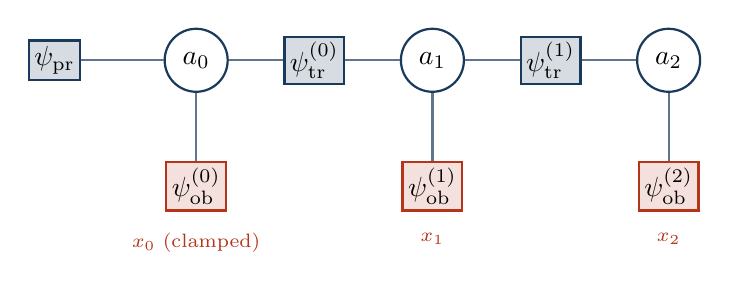
\begin{tikzpicture}[node distance=14mm]
  \node[var] (a0) at (0,0) {$a_0$};
  \node[var] (a1) at (3,0) {$a_1$};
  \node[var] (a2) at (6,0) {$a_2$};
  \node[fac] (pr) at (-1.8,0) {$\psi_{\mathrm{pr}}$};
  \node[fac] (t01) at (1.5,0) {$\psi^{(0)}_{\mathrm{tr}}$};
  \node[fac] (t12) at (4.5,0) {$\psi^{(1)}_{\mathrm{tr}}$};
  \node[obs] (o0) at (0,-1.6) {$\psi^{(0)}_{\mathrm{ob}}$};
  \node[obs] (o1) at (3,-1.6) {$\psi^{(1)}_{\mathrm{ob}}$};
  \node[obs] (o2) at (6,-1.6) {$\psi^{(2)}_{\mathrm{ob}}$};
  \draw[edge] (pr)--(a0); \draw[edge] (a0)--(t01)--(a1)--(t12)--(a2);
  \draw[edge] (a0)--(o0); \draw[edge] (a1)--(o1); \draw[edge] (a2)--(o2);
  \node[below=1.5mm of o0,accent,font=\scriptsize] {$x_0$ (clamped)};
  \node[below=1.5mm of o1,accent,font=\scriptsize] {$x_1$};
  \node[below=1.5mm of o2,accent,font=\scriptsize] {$x_2$};
\end{tikzpicture}
\caption{Factor graph of $p(a\given x)$ for $K=3$. Circles: variable (clean
frame) nodes. Blue squares: prior and transition factors. Red squares:
observation factors carrying the clamped data $x_k$. The graph is a
\emph{caterpillar tree}: a backbone $a_0$--$a_1$--$a_2$ with one leaf factor
per node.}
\label{fig:fg}
\end{figure}

\begin{proposition}[The graph is a tree]\label{prop:tree}
The factor graph of \eqref{eq:posterior} is connected and acyclic.
\end{proposition}

\begin{derivation}[\ref*{prop:tree}: counting edges]
Nodes: $K$ variables $+\,2K$ factors $=3K$. Edges: each transition factor has
degree $2$ ($2K{-}2$ edges), each observation factor degree $1$ ($K$ edges),
the prior degree $1$ ($1$ edge): total $3K-1$ = nodes $-\,1$. The graph is
connected (every $a_k$ is reachable from $a_0$ along the transition backbone),
and a connected graph with $V-1$ edges is a tree.
\end{derivation}

\begin{proposition}[Global Markov property]\label{prop:markov}
Conditioning on $a_k$ makes the left block
$(a_0,\dots,a_{k-1};x_0,\dots,x_{k-1})$ and the right block
$(a_{k+1},\dots,a_{K-1};x_{k+1},\dots,x_{K-1})$ independent: every path
between the blocks passes through $a_k$, and conditioning severs it.
\end{proposition}

\begin{intuition}[: this is exactly the geometry J.\ Garnier-Brun described]
The graph is ``very tree-like --- a straight line with things on the side.''
Every interior variable has degree three (two transitions, one observation);
every BP update will combine a \emph{small, fixed} number of incoming
messages. Two consequences, one per direction of the note: (i) BP is
\emph{exact} on trees \citep[Th.~14.1]{mezard2009information} --- no message
ever returns to its sender, so nothing is double-counted; (ii) this is the
\emph{opposite} of the dense, high-degree graphs for which AMP was built
(\S\ref{sec:amp}), which is where the BP/AMP contrast will come from.
\end{intuition}

% =============================================================================
\section{Belief propagation on the chain}\label{sec:bp}
% =============================================================================

\subsection{The sum--product rules}

On a generic factor graph, sum--product BP passes two kinds of message along
every edge --- variable-to-factor and factor-to-variable
\citep{mezard2009information,kschischang2001factor,pearl1988probabilistic}:
\begin{align}
  \nu_{i\to a}(a_i)&\ \propto\ \prod_{b\in\partial i\setminus a}\hat\nu_{b\to i}(a_i),
    \label{eq:vp-rule}\\
  \hat\nu_{a\to i}(a_i)&\ \propto\ \int \psi_a(a_{\partial a})
     \prod_{j\in\partial a\setminus i}\nu_{j\to a}(a_j)\ \dd a_{\partial a\setminus i},
    \label{eq:fp-rule}\\
  p(a_i)&\ \propto\ \prod_{a\in\partial i}\hat\nu_{a\to i}(a_i).
    \label{eq:belief-rule}
\end{align}
On a tree these equations have a unique solution reached in one inward and one
outward pass, and the beliefs \eqref{eq:belief-rule} are the \emph{exact}
marginals.

\subsection{Convention A on the chain, and the double-counting trap}

On the chain the rules collapse into one \emph{forward} and one
\emph{backward} sweep. The bookkeeping deserves care --- an earlier internal
version of these notes fell into a trap here, which the audit caught.

\begin{proposition}[Convention A]\label{prop:convA}
Define messages (functions of the receiving variable)
\begin{align}
  \mu_{\to 0}(a_0)&:=\psi_{\mathrm{pr}}(a_0), \label{eq:fwd-init}\\
  \mu_{\to k+1}(a_{k+1})
      &:=\int \psi^{(k)}_{\mathrm{tr}}(a_k,a_{k+1})\,\psi^{(k)}_{\mathrm{ob}}(a_k)\,
               \mu_{\to k}(a_k)\,\dd a_k, \label{eq:fwd-rec}\\
  \mu_{\leftarrow K-1}(a_{K-1})&:=1, \label{eq:bwd-init}\\
  \mu_{\leftarrow k-1}(a_{k-1})
      &:=\int \psi^{(k-1)}_{\mathrm{tr}}(a_{k-1},a_k)\,\psi^{(k)}_{\mathrm{ob}}(a_k)\,
               \mu_{\leftarrow k}(a_k)\,\dd a_k. \label{eq:bwd-rec}
\end{align}
Then, for every $k$,
\begin{equation}\label{eq:combine}
  p(a_k\given x)\ \propto\ \mu_{\to k}(a_k)\;\psi^{(k)}_{\mathrm{ob}}(a_k)\;
  \mu_{\leftarrow k}(a_k).
\end{equation}
The forward message into $a_k$ carries the evidence $x_0,\dots,x_{k-1}$
\emph{only}; the backward message carries $x_{k+1},\dots,x_{K-1}$
\emph{only}; the local evidence $\psi^{(k)}_{\mathrm{ob}}$ enters once, at
combination time.
\end{proposition}

\begin{derivation}[\ref*{prop:convA}: peeling the chain at $a_k$]
Integrate the joint \eqref{eq:posterior} over every $a_j$, $j\ne k$. By the
global Markov property (Proposition~\ref{prop:markov}) the integral splits at
$a_k$ into independent left and right halves; the local factor
$\psi^{(k)}_{\mathrm{ob}}(a_k)$ depends on no integrated variable and factors
out. \textbf{Left half:} define
$\mu_{\to k}(a_k):=\int\psi_{\mathrm{pr}}\prod_{u<k}\psi^{(u)}_{\mathrm{tr}}
\prod_{j<k}\psi^{(j)}_{\mathrm{ob}}\;\dd a_0\cdots\dd a_{k-1}$. Peeling the
innermost variable $a_{k-1}$ --- only three factors involve it --- yields
exactly the recursion \eqref{eq:fwd-rec}, with base case
\eqref{eq:fwd-init}. \textbf{Right half:} the mirror argument gives
\eqref{eq:bwd-rec}--\eqref{eq:bwd-init}; the base case is flat because there
is no evidence to the right of the last frame. \textbf{Combination:} left
integral $\times$ local evidence $\times$ right integral is
\eqref{eq:combine}, with normaliser $P_t(x)$.
\end{derivation}

\begin{remark}[The double-counting trap]\label{rmk:trap}
A natural-looking alternative (\emph{Convention~B}) absorbs the local
evidence into the forward message,
$\mu^{\mathrm B}_{\to k}:=\mu^{\mathrm A}_{\to k}\cdot\psi^{(k)}_{\mathrm{ob}}$.
Under Convention~B the simple product \eqref{eq:combine} counts $x_k$
\emph{twice} --- once inside the message, once at combination --- and must be
corrected by dividing one factor back out. Convention~A is the bookkeeping
under which the textbook combination rule is correct \emph{as written}. The
audit was decisive in pinning this down: under Convention~A the BP score
matches the matrix score to $10^{-14}$; under naive Convention~B the
disagreement is order one. This is the single most error-prone point of the
whole construction, and the reason every formula in this section is stated
with its evidence bookkeeping made explicit.
\end{remark}

\subsection{Complexity}

Each sweep computes $K-1$ messages, each by a single one-dimensional integral;
the combination at each node is a product of three one-variable functions.
Total: $2(K-1)$ integrals $+\ K$ combinations $=O(K)$, against $O(K^2)$ for
direct per-marginal elimination and $O(K^3)$ for matrix inversion. For the
Gaussian model each ``integral'' is two arithmetic operations on
$(\lambda,\theta)$ pairs, so the constant is tiny as well.

% =============================================================================
\section{BP on the $K=3$ chain: every message, by hand}\label{sec:bp3}
% =============================================================================

We now execute \eqref{eq:fwd-init}--\eqref{eq:combine} on Fig.~\ref{fig:fg},
first symbolically, then numerically on a concrete instance. Every message is
Gaussian (the integrals are instances of Lemmas \ref{lem:product} and
\ref{lem:predict}), so each is carried by a (mean, variance) pair.

\subsection{The local evidence as a Gaussian in $a_k$}

Read as a function of $a_k$, the observation factor is
\begin{equation}\label{eq:obs-info}
  \psi^{(k)}_{\mathrm{ob}}(a_k)=\N(x_k;e^{-t}a_k,\Dt)\ \propto\
  \exp\!\Big(-\tfrac12\,\tfrac{e^{-2t}}{\Dt}\,a_k^2
  +\tfrac{e^{-t}}{\Dt}x_k\,a_k\Big)
  \;\;\Longleftrightarrow\;\;
  \N\!\big(a_k;\;e^{t}x_k,\;\Dt e^{2t}\big),
\end{equation}
a Gaussian \emph{pseudo-observation} of $a_k$ at the deconvolved location
$e^tx_k$ with variance $\Dt e^{2t}$ (precision $e^{-2t}/\Dt$: the pinning
strength of the tilted-measure box in \S\ref{sec:noisy}).

\subsection{Forward sweep = predict--update filter}

\begin{derivation}[: forward sweep (Convention A)]
\textbf{Initialisation.} $\mu_{\to0}=\psi_{\mathrm{pr}}=\N(a_0;0,1)$.

\textbf{Generic step $k\to k+1$.} Two half-steps:
\begin{itemize}[leftmargin=1.6em, topsep=2pt, itemsep=2pt]
\item \emph{Update} (Lemma~\ref{lem:product}): combine the incoming message
with the local evidence \eqref{eq:obs-info},
\[
  \N(m^{\to}_k,v^{\to}_k)\times\N(e^tx_k,\Dt e^{2t})
  \ \longrightarrow\
  \N(m^c_k,v^c_k),\qquad
  \frac1{v^c_k}=\frac1{v^{\to}_k}+\frac{e^{-2t}}{\Dt},\quad
  \frac{m^c_k}{v^c_k}=\frac{m^{\to}_k}{v^{\to}_k}+\frac{e^{-t}}{\Dt}x_k .
\]
\item \emph{Predict} (Lemma~\ref{lem:predict}): push through the transition,
\[
  \mu_{\to k+1}=\int\N(a_{k+1};\alpha a_k,\sigma_\eta^2)\,
   \N(a_k;m^c_k,v^c_k)\,\dd a_k
  =\N\!\big(a_{k+1};\ \alpha m^c_k,\ \alpha^2v^c_k+\sigma_\eta^2\big).
\]
\end{itemize}
This is precisely the predict--update cycle of the \emph{Kalman filter}
\citep{kalman1960}: BP on a Gaussian chain \emph{is} Kalman filtering.
\end{derivation}

\begin{derivation}[: backward sweep]
Start flat, $\mu_{\leftarrow K-1}\equiv1$ ($\lambda=0$). Generic step
$k\to k-1$: combine $\mu_{\leftarrow k}$ with the local evidence at $k$
(Lemma~\ref{lem:product}) to get $\N(m^c_k,v^c_k)$, then invert the transition
$a_k=\alpha a_{k-1}+\eta$:
\[
  \mu_{\leftarrow k-1}
  =\int\N(a_k;\alpha a_{k-1},\sigma_\eta^2)\,\N(a_k;m^c_k,v^c_k)\,\dd a_k
  =\N\!\Big(a_{k-1};\ \frac{m^c_k}{\alpha},\
   \frac{v^c_k+\sigma_\eta^2}{\alpha^2}\Big),
\]
because viewing the integrand as a function of $a_{k-1}$, the exponent is
quadratic with the stated mean and variance (equivalently: apply
Lemma~\ref{lem:predict} to the inverted relation
$a_{k-1}=(a_k-\eta)/\alpha$).
\end{derivation}

\begin{derivation}[: combination $=$ RTS smoother]
At each node, \eqref{eq:combine} multiplies three Gaussians
(Lemma~\ref{lem:product} twice):
\[
  p(a_k\given x)=\N\!\big(m^{\mathrm{post}}_k,v^{\mathrm{post}}_k\big),\qquad
  \frac1{v^{\mathrm{post}}_k}=\frac1{v^{\to}_k}+\frac{e^{-2t}}{\Dt}
  +\frac1{v^{\leftarrow}_k},\qquad
  \frac{m^{\mathrm{post}}_k}{v^{\mathrm{post}}_k}
  =\frac{m^{\to}_k}{v^{\to}_k}+\frac{e^{-t}}{\Dt}x_k
  +\frac{m^{\leftarrow}_k}{v^{\leftarrow}_k}.
\]
The forward--backward combination is the \emph{Rauch--Tung--Striebel
smoother} \citep{rauchtungstriebel1965}. Substituting
$m^{\mathrm{post}}_k$ into Tweedie \eqref{eq:tweedie} gives the $k$-th score
component.
\end{derivation}

\begin{figure}[h]\centering
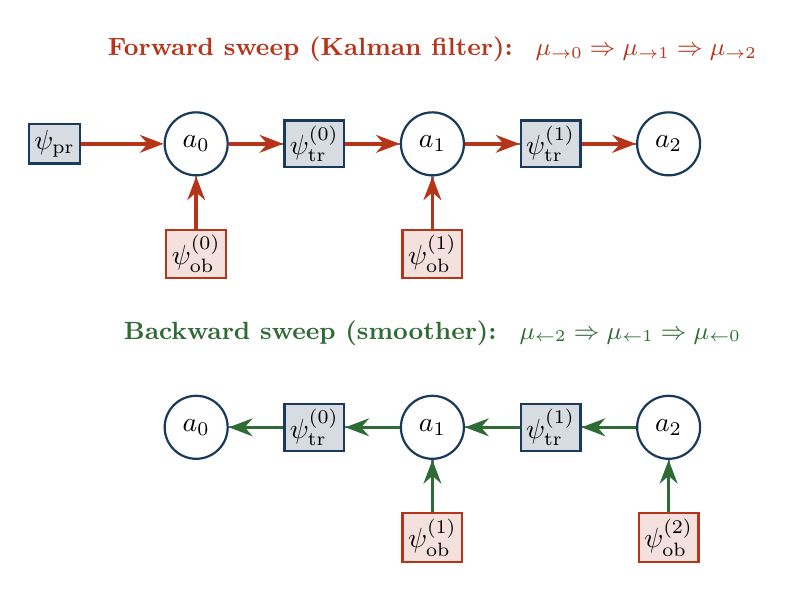
\begin{tikzpicture}[node distance=14mm]
  % forward
  \begin{scope}
  \node[var] (a0) at (0,0) {$a_0$};
  \node[var] (a1) at (3,0) {$a_1$};
  \node[var] (a2) at (6,0) {$a_2$};
  \node[fac] (pr) at (-1.8,0) {$\psi_{\mathrm{pr}}$};
  \node[fac] (t01) at (1.5,0) {$\psi^{(0)}_{\mathrm{tr}}$};
  \node[fac] (t12) at (4.5,0) {$\psi^{(1)}_{\mathrm{tr}}$};
  \node[obs] (o0) at (0,-1.4) {$\psi^{(0)}_{\mathrm{ob}}$};
  \node[obs] (o1) at (3,-1.4) {$\psi^{(1)}_{\mathrm{ob}}$};
  \draw[edge] (a0)--(t01)--(a1)--(t12)--(a2);
  \draw[edge] (a0)--(o0); \draw[edge] (a1)--(o1);
  \draw[fwd] (pr)--(a0); \draw[fwd] (a0)--(t01);
  \draw[fwd] (t01)--(a1); \draw[fwd] (a1)--(t12); \draw[fwd] (t12)--(a2);
  \draw[fwd] (o0)--(a0); \draw[fwd] (o1)--(a1);
  \node[font=\bfseries\small,accent] at (3,1.2)
    {Forward sweep (Kalman filter): $\ \mu_{\to0}\Rightarrow\mu_{\to1}\Rightarrow\mu_{\to2}$};
  \end{scope}
  % backward
  \begin{scope}[yshift=-3.6cm]
  \node[var] (b0) at (0,0) {$a_0$};
  \node[var] (b1) at (3,0) {$a_1$};
  \node[var] (b2) at (6,0) {$a_2$};
  \node[fac] (s01) at (1.5,0) {$\psi^{(0)}_{\mathrm{tr}}$};
  \node[fac] (s12) at (4.5,0) {$\psi^{(1)}_{\mathrm{tr}}$};
  \node[obs] (p1) at (3,-1.4) {$\psi^{(1)}_{\mathrm{ob}}$};
  \node[obs] (p2) at (6,-1.4) {$\psi^{(2)}_{\mathrm{ob}}$};
  \draw[edge] (b0)--(s01)--(b1)--(s12)--(b2);
  \draw[edge] (b1)--(p1); \draw[edge] (b2)--(p2);
  \draw[bwd] (b2)--(s12); \draw[bwd] (s12)--(b1);
  \draw[bwd] (b1)--(s01); \draw[bwd] (s01)--(b0);
  \draw[bwd] (p2)--(b2); \draw[bwd] (p1)--(b1);
  \node[font=\bfseries\small,intuiframe] at (3,1.2)
    {Backward sweep (smoother): $\ \mu_{\leftarrow2}\Rightarrow\mu_{\leftarrow1}\Rightarrow\mu_{\leftarrow0}$};
  \end{scope}
\end{tikzpicture}
\caption{The two sweeps for $K=3$, drawn on the factor nodes. Forward (red):
information from the prior and from $x_0,x_1$ flows left to right; the
forward message into $a_k$ has already absorbed $x_0,\dots,x_{k-1}$ (and not
$x_k$: Convention~A). Backward (green): information from $x_2,x_1$ flows
right to left. The posterior at $a_k$ multiplies forward message, local
evidence, and backward message --- each observation counted exactly once.}
\label{fig:sweeps}
\end{figure}

\subsection{A complete numerical instance}

Fix $\alpha=0.7$, $t=0.5$, $x=(1.2,\,-0.4,\,0.8)$. Then
\[
  e^{-t}=0.606531,\quad \Dt=0.632121,\quad \sigma_\eta^2=0.51,\quad
  \tfrac{e^{-2t}}{\Dt}=0.581977,\quad \tfrac{e^{-t}}{\Dt}=0.959517 .
\]
The pseudo-observations \eqref{eq:obs-info} are
$\N(e^tx_k,\,\Dt e^{2t})=\N(1.648721\,x_k,\;1.718282)$. Executing the sweeps:

\begin{center}\small
\begin{tabular}{@{}lccc@{}}
\toprule
message & at $a_0$ & at $a_1$ & at $a_2$\\
\midrule
forward $\mu_{\to k}$ (mean, var) & $(0,\ 1)$ & $(+0.509486,\ 0.819739)$ & $(+0.092348,\ 0.781939)$\\
evidence \eqref{eq:obs-info} (mean, var) & $(+1.978466,\ 1.718282)$ & $(-0.659489,\ 1.718282)$ & $(+1.318977,\ 1.718282)$\\
backward $\mu_{\leftarrow k}$ (mean, var) & $(+0.054410,\ 3.585865)$ & $(+1.884253,\ 4.547514)$ & flat ($\lambda=0$)\\
\midrule
posterior (mean, var) & $(+0.626915,\ 0.537389)$ & $(+0.322520,\ 0.494614)$ & $(+0.475974,\ 0.537389)$\\
\bottomrule
\end{tabular}
\end{center}

\noindent Sample hand-checks (all reproduced in notebook
\texttt{02\_belief\_propagation}):
\begin{itemize}[leftmargin=1.6em, itemsep=1pt]
\item \emph{Forward at $a_1$}: combine $(0,1)$ with the evidence at node $0$:
precision $1+0.581977=1.581977$, variance $0.632121$, mean
$0.632121\times(0+0.959517\times1.2)=0.727846$; predict:
mean $0.7\times0.727846=0.509492$, variance
$0.49\times0.632121+0.51=0.819739$. \;(Matches the table to rounding.)
\item \emph{Backward at $a_1$}: combine flat with evidence at node $2$:
$(1.318977,1.718282)$; invert the transition: mean $1.318977/0.7=1.884253$,
variance $(1.718282+0.51)/0.49=4.547514$. \;\checkmark
\item \emph{Posterior at $a_1$}: add the three precisions
$1/0.819739+0.581977+1/4.547514=2.021779$, variance $0.494614$; the mean
follows from the potentials. \;\checkmark
\end{itemize}
The matrix route \eqref{eq:posterior-J} gives posterior mean
$(0.626915,\,0.322520,\,0.475974)$ and variances
$(0.537389,\,0.494614,\,0.537389)$ --- identical. Tweedie
\eqref{eq:tweedie} then yields the score
\[
  S(x,0.5)=(-1.296836,\ +0.942254,\ -0.808876),
\]
which equals $-\Qt x$ from \eqref{eq:score-matrix} to machine precision.
Note the sign of $S_1$: although $x_1=-0.4$ is negative, its neighbours pull
the posterior mean of $a_1$ \emph{positive} ($+0.32$), so the score pushes
$x_1$ \emph{up} --- a purely joint effect, impossible for the marginal score
$-x_1$ to produce\ldots\ this is Remark~\ref{rmk:joint} in numbers.

% =============================================================================
\section{General $K$: Gaussian closure and the Kalman connection}\label{sec:bpK}
% =============================================================================

For general $K$ nothing changes: the recursions
\eqref{eq:fwd-rec}--\eqref{eq:bwd-rec} run for $K-1$ steps each, and the
combination \eqref{eq:combine} holds at every node. Each sweep is a sequence
of update (Lemma~\ref{lem:product}) and predict (Lemma~\ref{lem:predict})
operations on $(\lambda,\theta)$ pairs.

\begin{theorem}[Gaussian closure --- answering ``are the messages
Gaussian?'']\label{thm:closure}
For the model \eqref{eq:ar1}--\eqref{eq:ou}, every BP message and every belief
is \emph{exactly} Gaussian, at every node, for every $K$, $\alpha$, $t$;
consequently the posterior marginals are Gaussian, and BP computes them
exactly.
\end{theorem}

\begin{derivation}[\ref*{thm:closure}]
By induction along each sweep. The initial messages are Gaussian
(\eqref{eq:fwd-init}: the prior; \eqref{eq:bwd-init}: the flat limit
$\lambda\to0$ of a Gaussian family). Each recursion step consists of one
product of Gaussians in the same variable (Lemma~\ref{lem:product}) and one
Gaussian propagation (Lemma~\ref{lem:predict}), both of which return
Gaussians. The combination \eqref{eq:combine} is a product of three Gaussians.
Exactness then follows from tree-exactness of BP
(Proposition~\ref{prop:tree} and \citep[Th.~14.1]{mezard2009information}).
\qed
\end{derivation}

\begin{intuition}[: closure is algebra, not a central limit theorem]
The closure holds at every node degree --- on the degree-$2$ chain just as on
a dense graph --- because it is a property of the Gaussian \emph{family} under
multiplication and affine marginalisation, not of any aggregation of many
weak influences. This resolves the doubt raised in discussion: no CLT is
invoked anywhere, so there is no ``CLT on two points'' to fail \emph{for BP}.
The CLT enters only when one tries to justify the \emph{AMP} closure
(\S\ref{sec:amp}) --- and there, on the chain, it does fail, exactly as
anticipated.
\end{intuition}

\begin{intuition}[: the classical identifications]
Forward sweep $=$ Kalman filter \citep{kalman1960}; forward$+$backward
combination $=$ Rauch--Tung--Striebel smoother \citep{rauchtungstriebel1965};
both are the Gaussian specialisation of sum--product on the chain
\citep{kschischang2001factor,bishop2006pattern}. Tweedie
\eqref{eq:tweedie} then says: \emph{the $k$-th joint score component is an
affine function of the Kalman-smoothed estimate of frame $k$} --- the joint
score of a Markov sequence is a smoothing problem, solved in $O(K)$.
\end{intuition}

\begin{auditbox}[: BP reproduces the matrix posterior and the exact score]
\texttt{numerical\_audit.py} sweeps $K\in\{2,3,5,8,16\}$,
$\alpha\in\{0.2,0.5,0.9,-0.4\}$, $t\in\{0.05,0.3,1,3\}$ (80 configurations,
random $x$): maximum disagreement between BP and the matrix route
\eqref{eq:posterior-J} is $1.3\times10^{-15}$ (means),
$3.9\times10^{-15}$ (variances), $1.2\times10^{-14}$ (scores) ---
double-precision rounding accumulated along the recursion. BP \emph{is} the
score, computed through the precision matrix in $O(K)$.
\end{auditbox}

% =============================================================================
\section{The chain solved in closed form: bulk analysis}\label{sec:bulk}
% =============================================================================

So far BP is an \emph{algorithm}; in this section we solve its fixed point in
closed form in the \emph{bulk} of the chain --- the homogeneous interior of a
long chain, far from both boundaries --- and obtain explicit formulas for the
posterior variance, the full posterior covariance, and the correlation length
of the score. These formulas are the backbone of the BP/AMP comparison
(\S\ref{sec:amp}) and of Experiment~A (\S\ref{sec:expA}).

\subsection{Bulk parameters}

In the interior, the posterior precision \eqref{eq:posterior-J} is the
tridiagonal Toeplitz matrix with
\begin{equation}\label{eq:bulk-params}
  \boxed{\ \Jd=\frac{e^{-2t}}{\Dt}+\frac{1+\alpha^2}{\sigma_\eta^2},
  \qquad
  \beta=-\frac{\alpha}{\sigma_\eta^2}\ }\qquad(\sigma_\eta^2=1-\alpha^2).
\end{equation}
$\Jd$ has two parts with opposite behaviour in $t$: the \emph{evidence}
precision $e^{-2t}/\Dt$ (the tilted-measure pinning strength, divergent as
$1/2t$ at small $t$, vanishing at large $t$) and the \emph{prior} precision
$(1+\alpha^2)/\sigma_\eta^2$ (constant). The coupling $\beta$ is pure prior.
The single dimensionless ratio $|\beta|/\Jd\in(0,\tfrac12)$ controls
everything below.

\subsection{The BP fixed point and the exact bulk variance}

Write Gaussian BP directly in the $(J,h)$ parametrisation: the message from
node $k$ to node $k{+}1$ is Gaussian with some precision, and on the
homogeneous interior the precision $\lambda_k$ of the \emph{one-sided summary}
(everything to the left of $k{+}1$, evidence included) obeys
\begin{equation}\label{eq:cavity-rec}
  \lambda_{k+1}=\Jd-\frac{\beta^2}{\lambda_k},
\end{equation}
obtained by integrating $a_k$ out of
$\exp(-\tfrac12\lambda_ka_k^2+\theta_ka_k-\beta a_ka_{k+1}-\dots)$: the
Gaussian integral contributes $-\beta^2/\lambda_k$ to the precision seen by
$a_{k+1}$. (This is the same algebra as \S\ref{sec:bp3} in a different
parametrisation; the audit checks the \emph{results} agree.)

\begin{theorem}[BP bulk fixed point --- always exists]\label{thm:bp-bulk}
The recursion \eqref{eq:cavity-rec} has the fixed points
$\lambda^\pm=(\Jd\pm\sqrt{\Jd^2-4\beta^2})/2$. For every $\alpha\in(-1,1)$ and
every $t>0$,
\[
  \Jd-2|\beta|\;=\;\frac{e^{-2t}}{\Dt}+\frac{(1-|\alpha|)^2}{\sigma_\eta^2}\;>\;0,
\]
so the discriminant is strictly positive, the upper fixed point
\begin{equation}\label{eq:bp-fixed}
  \boxed{\ \lambda^\ast=\frac{\Jd+\sqrt{\Jd^2-4\beta^2}}{2}\ }
\end{equation}
exists, and it is strictly attractive
($|f'(\lambda^\ast)|=\beta^2/\lambda^{\ast2}<1$). Recombining the two
directions and the local term,
\begin{equation}\label{eq:bulk-var}
  \Lambda_{\mathrm{bulk}}
  =\Jd-\frac{\beta^2}{\lambda^\ast}-\frac{\beta^2}{\lambda^\ast}
  =\sqrt{\Jd^2-4\beta^2}
  \qquad\Longrightarrow\qquad
  \boxed{\ V_{\mathrm{exact}}=\frac{1}{\sqrt{\Jd^2-4\beta^2}}\ }
\end{equation}
\end{theorem}

\begin{derivation}[\ref*{thm:bp-bulk}]
\textbf{Existence.} $1+\alpha^2-2|\alpha|=(1-|\alpha|)^2\ge0$ (AM--GM, with
equality only at $|\alpha|=1$, excluded), and the evidence term is positive
for every finite $t$; hence $\Jd>2|\beta|$ strictly and the square root is
real. \textbf{Stability.} The map $f(\lambda)=\Jd-\beta^2/\lambda$ has
$f'(\lambda)=\beta^2/\lambda^2$; since
$\lambda^\ast\ge\Jd/2>|\beta|$, we get $f'(\lambda^\ast)<1$: the forward sweep
converges geometrically to $\lambda^\ast$ from any positive initialisation,
and the boundary effects of a finite chain decay at the same geometric rate.
\textbf{Recombination.} The marginal precision at a bulk node is the local
$\Jd$ plus the two one-sided corrections $-\beta^2/\lambda^\ast$. Using
$\lambda^{\ast2}-\Jd\lambda^\ast+\beta^2=0$, i.e.\
$\beta^2/\lambda^\ast=\Jd-\lambda^\ast$:
$\Lambda_{\mathrm{bulk}}=\Jd-2(\Jd-\lambda^\ast)=2\lambda^\ast-\Jd
=\sqrt{\Jd^2-4\beta^2}$. \qed
\end{derivation}

\subsection{The full bulk covariance and the correlation length of the score}

\begin{theorem}[Geometric posterior covariance]\label{thm:bulk-cov}
In the bulk, the posterior covariance decays geometrically with frame
distance:
\begin{equation}\label{eq:bulk-cov}
  \boxed{\ (J^{-1})_{i,\,i+d}=\frac{q^{\,d}}{\sqrt{\Jd^2-4\beta^2}},\qquad
  q=\frac{\Jd-\sqrt{\Jd^2-4\beta^2}}{2\,|\beta|}\in(0,1).\ }
\end{equation}
\end{theorem}

\begin{derivation}[\ref*{thm:bulk-cov}: transfer-matrix ansatz]
For an infinite tridiagonal Toeplitz $J$, seek the row of the inverse in the
form $(J^{-1})_{i,i+d}=C\,q^{\,d}$ for $d\ge0$ (symmetric in $d$). The
defining relation $\sum_j J_{ij}(J^{-1})_{j,i+d}=\delta_{0d}$ reads, for
$d\ge1$,
\[
  \beta\,Cq^{\,d-1}+\Jd\,Cq^{\,d}+\beta\,Cq^{\,d+1}=0
  \quad\Longleftrightarrow\quad
  \beta q^2+\Jd q+\beta=0 ,
\]
whose root inside the unit disc is $q=(\Jd-\sqrt{\Jd^2-4\beta^2})/(2|\beta|)$
(for $\beta<0$, i.e.\ $\alpha>0$, the inverse entries are all positive; for
$\alpha<0$ they alternate in sign, $q\mapsto-q$, with the same modulus). The
$d=0$ relation fixes
$C$: $\Jd C+2\beta Cq=1$ and $2\beta q=-(\Jd-\sqrt{\Jd^2-4\beta^2})$ give
$C=1/\sqrt{\Jd^2-4\beta^2}=V_{\mathrm{exact}}$, consistently with
\eqref{eq:bulk-var}. \qed
\end{derivation}

\begin{intuition}[: $q$ is the memory of the posterior --- with the right limits]
$q$ measures how far evidence travels along the chain: the posterior
correlation length is $\xi=1/\log(1/q)$ frames. Its limits are exactly what
they must be:
\[
  t\to0:\quad q\approx\frac{|\beta|}{\Jd}\to0
  \quad\text{(each frame pinned by its own data: near-diagonal posterior)};
\]
\[
  t\to\infty:\quad
  q\to\frac{(1+\alpha^2)-(1-\alpha^2)}{2|\alpha|}=|\alpha|
  \quad\text{(no data: the posterior \emph{is} the prior)}.
\]
So as diffusion time runs, the score's internal correlation length climbs
monotonically from $0$ to the prior's own $1/\log(1/|\alpha|)$. This single
number $q(\alpha,t)$ will reappear as the \emph{exact decay rate of the
locality error} in Experiment~A.
\end{intuition}

\begin{auditbox}[: bulk formulas vs brute force]
At the centre of a $K=400$ chain, over $20$ configurations
($\alpha\in\{0.2,0.5,0.8,0.95,-0.6\}$, $t\in\{0.05,0.3,1,3\}$):
$V_{\mathrm{exact}}$ matches $\diag(J^{-1})$ to relative error
$2.2\times10^{-11}$; the geometric law \eqref{eq:bulk-cov} matches
$(J^{-1})_{i,i+d}$ for $d\le5$ to $8.1\times10^{-13}$; the recombination
identity in \eqref{eq:bulk-var} holds to $1.4\times10^{-14}$ on a
$2010$-point $(\alpha,t)$ grid; and the existence margin $\Jd-2|\beta|$ is
positive over the entire grid.
\end{auditbox}

% =============================================================================
\section{Approximate message passing: same score, different variance,
explicit breakdown}\label{sec:amp}
% =============================================================================

\subsection{The general idea, and why our model is its opposite}

AMP --- in the physics literature, the TAP equations --- is the message
passing one uses when exact messages cannot be tracked and the factor graph is
\emph{dense} \citep{zdeborova2021statistical,donoho2009message,
mezard2009information}. For a linear model $y=\Phi a+w$ with dense
$\Phi\in\R^{m\times N}$, every factor touches all $N$ variables; each message
is then a sum of many weakly dependent contributions, hence \emph{approximately
Gaussian by a central limit argument}, and one propagates only means and
variances, with the Onsager reaction term subtracting each node's
back-influence. Rigorously, \citet{genovese2026amp} show for $\ell_2$
minimisation that the BP means satisfy the AMP equations asymptotically as
$N\to\infty$ --- and note that on a \emph{tree} BP is already exact, so AMP
has nothing to add there.

Our model is the opposite of this regime in every respect: the measurement
operator is \emph{diagonal} ($x=e^{-t}a+\text{noise}$), the coupling lives in
the \emph{prior}, and every node has at most two neighbours. To make the
comparison concrete we view the posterior \eqref{eq:posterior-J} as a Gaussian
Markov random field with precision $J$ and field $h$ and ask three solvers
for its marginals:
\[
 \text{mean field: } V_i=\tfrac1{J_{ii}};\qquad
 \text{AMP/TAP: } V_i=\frac{1}{J_{ii}-\sum_{k\ne i}J_{ik}^2 V_k};\qquad
 \text{BP/exact: } V_i=(J^{-1})_{ii}.
\]
The AMP/TAP closure is the cavity variance with the ``exclude one neighbour''
correction dropped ($V_{k\to i}\approx V_k$): harmless when each node has many
weak neighbours (removing one is an $O(1/N)$ change --- the dense regime), an
$O(1)$ modification on a chain where each node has two.

\subsection{The score is closure-independent}

\begin{theorem}[Same mean $\Rightarrow$ same score]\label{thm:same-score}
For a Gaussian posterior, the stationarity condition for the mean is the
\emph{same} linear system $Jm=h$ under mean field, BP, and AMP. Hence all
three return the exact posterior mean, and --- via Tweedie
\eqref{eq:tweedie} --- the \emph{same, exact, joint score}, for every
$(K,\alpha,t)$, regardless of whether the variance closure is accurate or even
solvable.
\end{theorem}

\begin{derivation}[\ref*{thm:same-score}]
In each scheme the update for the mean of node $i$ has the form
$m_i\leftarrow(h_i-\sum_{k\ne i}J_{ik}\,m_{k})/J_{ii}$ (with
scheme-dependent corrections that vanish at the fixed point: the cavity
exclusion affects which $V$'s appear, not the linear relation among the
means). At any fixed point, $J_{ii}m_i+\sum_{k\ne i}J_{ik}m_k=h_i$ for all
$i$, i.e.\ $Jm=h$, whose unique solution is the exact posterior mean. The
variance closure modifies only the \emph{uncertainty} bookkeeping. Tweedie
converts the mean into the score; the score is therefore closure-independent.
\qed
\end{derivation}

\begin{intuition}[: why this is the precise answer to ``is AMP $=$ BP here?'']
For the \emph{score} --- the object diffusion actually needs --- yes: BP, AMP
and even naive mean field coincide, because the score only needs the
posterior mean and the mean solves a closure-independent linear system. For
the \emph{posterior variances} --- the object that message-passing theory
needs internally (and that controls error bars, likelihoods, and any
nonlinear extension) --- no: the closures differ, measurably and, as we now
show, catastrophically at strong coupling.
\end{intuition}

\subsection{The AMP bulk fixed point, its breakdown time, and the critical
coupling}

In the bulk, the AMP closure reads $V=1/(\Jd-2\beta^2V)$ --- compare the BP
cavity $V_{\mathrm{cav}}=1/(\Jd-\beta^2V_{\mathrm{cav}})$
of \eqref{eq:cavity-rec}: \emph{the entire difference between BP and AMP on
the chain is the factor 2}, both neighbours included where BP excludes one.

\begin{theorem}[AMP bulk variance and existence]\label{thm:amp-bulk}
The AMP closure is the quadratic $2\beta^2V^2-\Jd V+1=0$, with physical root
\begin{equation}\label{eq:amp-fixed}
  \boxed{\ V_{\textsc{amp}}
  =\frac{\Jd-\sqrt{\Jd^2-8\beta^2}}{4\beta^2}\ }
\end{equation}
(the branch continuously connected to the decoupled limit $1/\Jd$ as
$\beta\to0$), which exists \emph{iff}
\begin{equation}\label{eq:amp-exists}
  \boxed{\ \Jd\ \ge\ 2\sqrt2\,|\beta|\ }
\end{equation}
--- a strictly stronger requirement than BP's $\Jd\ge2|\beta|$
(Theorem~\ref{thm:bp-bulk}), which always holds. Solving
\eqref{eq:amp-exists} as an equality for $t$, with
$u:=e^{-2t}$ and $e^{-2t}/\Dt=u/(1-u)$:
\begin{equation}\label{eq:tc}
  t_c(\alpha)=-\tfrac12\log\frac{g}{1+g},\qquad
  g(\alpha)=\frac{2\sqrt2\,|\alpha|-1-\alpha^2}{1-\alpha^2},
\end{equation}
finite exactly when $g>0$, i.e.\
\begin{equation}\label{eq:alphac}
  \boxed{\ |\alpha|>\alpha_c=\sqrt2-1\approx0.4142\ }
\end{equation}
For $|\alpha|\le\alpha_c$ the AMP variance has a fixed point at \emph{every}
diffusion time; for $|\alpha|>\alpha_c$ it ceases to exist for all
$t>t_c(\alpha)$.
\end{theorem}

\begin{derivation}[\ref*{thm:amp-bulk}]
\textbf{Quadratic and branch.} Multiply $V(\Jd-2\beta^2V)=1$ out; the roots
are $V_\pm=(\Jd\pm\sqrt{\Jd^2-8\beta^2})/(4\beta^2)$. As $\beta\to0$,
$V_-\to1/\Jd$ (expand the square root) while $V_+$ diverges; moreover $V_-$ is
the attractive fixed point of the damped iteration used in practice. Real
roots require $\Jd^2\ge8\beta^2$. \textbf{Breakdown time.} The map
$t\mapsto\Jd(t)$ is strictly decreasing (the evidence dies as $t$ grows) with
range $(\,(1{+}\alpha^2)/\sigma_\eta^2,\ \infty)$, so the equality
$\Jd=2\sqrt2|\beta|$ has at most one solution. Substituting $u/(1-u)$ for the
evidence term and solving the linear equation in $u$ gives \eqref{eq:tc}.
\textbf{Critical coupling.} $g>0\iff\alpha^2-2\sqrt2|\alpha|+1<0
\iff|\alpha|\in(\sqrt2-1,\sqrt2+1)$; with $|\alpha|<1$ this is
$|\alpha|>\sqrt2-1$. Equivalently: at $t=\infty$ the posterior is the bare
prior, $J\to Q_0$, and \eqref{eq:amp-exists} for $Q_0$ itself reads
$(1+\alpha^2)\ge2\sqrt2|\alpha|$ --- AMP applied to a bare \textsc{ar}(1)
chain works iff $|\alpha|\le\sqrt2-1$. \qed
\end{derivation}

\begin{theorem}[Weak-coupling law: AMP errs at fourth order, upward]
\label{thm:weak}
Expanding \eqref{eq:bulk-var} and \eqref{eq:amp-fixed} in
$\epsilon:=\beta^2/\Jd^2$,
\[
  V_{\mathrm{exact}}=\frac1\Jd\big(1+2\epsilon+6\epsilon^2+O(\epsilon^3)\big),
  \qquad
  V_{\textsc{amp}}=\frac1\Jd\big(1+2\epsilon+8\epsilon^2+O(\epsilon^3)\big),
\]
so the closures agree to second order in the coupling and
\begin{equation}\label{eq:weak}
  \boxed{\ V_{\textsc{amp}}-V_{\mathrm{exact}}
  =\frac{2\beta^4}{\Jd^5}+O\!\Big(\frac{\beta^6}{\Jd^7}\Big)\ }\qquad
  \text{--- AMP always \emph{over}estimates the bulk variance.}
\end{equation}
\end{theorem}

\begin{derivation}[\ref*{thm:weak}]
$(1-4\epsilon)^{-1/2}=1+2\epsilon+6\epsilon^2+O(\epsilon^3)$ gives the exact
expansion. For AMP, $1-\sqrt{1-8\epsilon}
=4\epsilon+8\epsilon^2+O(\epsilon^3)$, and multiplying by
$\Jd/(4\beta^2)=1/(4\epsilon\Jd)$ gives the stated series. Subtracting,
$V_{\textsc{amp}}-V_{\mathrm{exact}}=2\epsilon^2/\Jd=2\beta^4/\Jd^5$ at
leading order. \qed
\end{derivation}

\begin{figure}[h]\centering
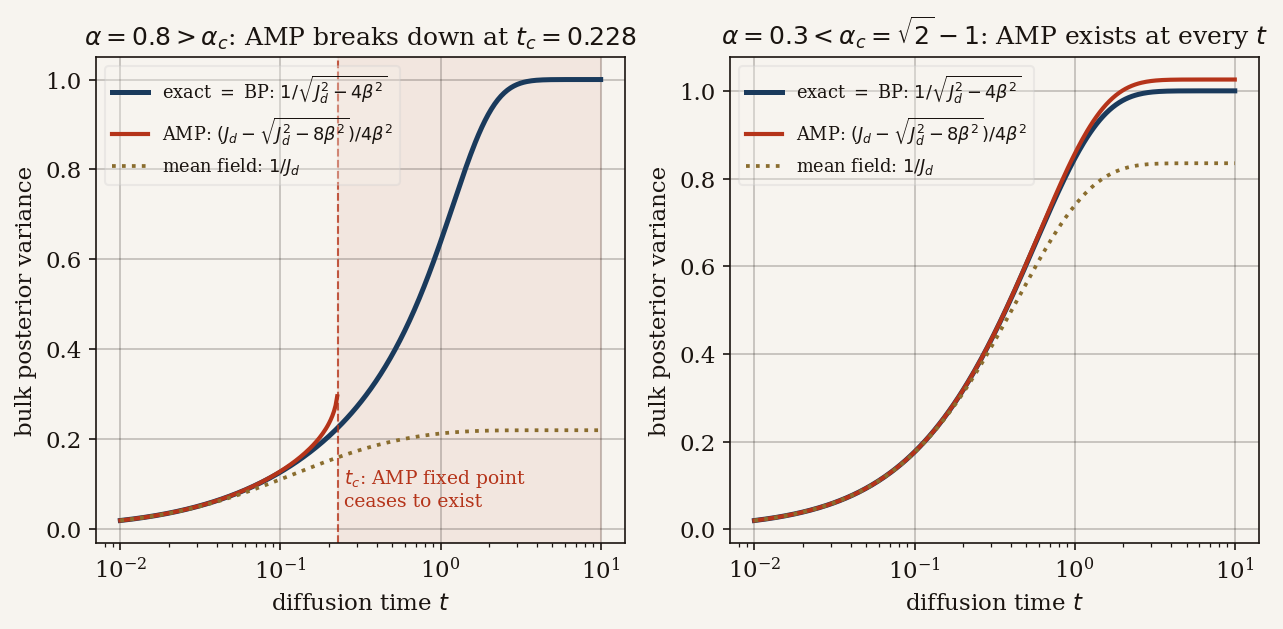
\includegraphics[width=\linewidth]{figures/fig_bulk_variance.png}
\caption{\textbf{Bulk posterior variance: the three closures in closed form.}
Left ($\alpha=0.8>\alpha_c$): exact $=$ BP (navy), AMP \eqref{eq:amp-fixed}
(red), mean field (gold). The AMP branch terminates with the characteristic
square-root singularity at the exact breakdown time
$t_c(0.8)=0.228$ from \eqref{eq:tc} (shaded: no fixed point). Right
($\alpha=0.3<\alpha_c$): AMP exists at every $t$ and slightly overestimates
the variance at large $t$, as predicted by \eqref{eq:weak}.}
\label{fig:bulkvar}
\end{figure}

\begin{figure}[h]\centering
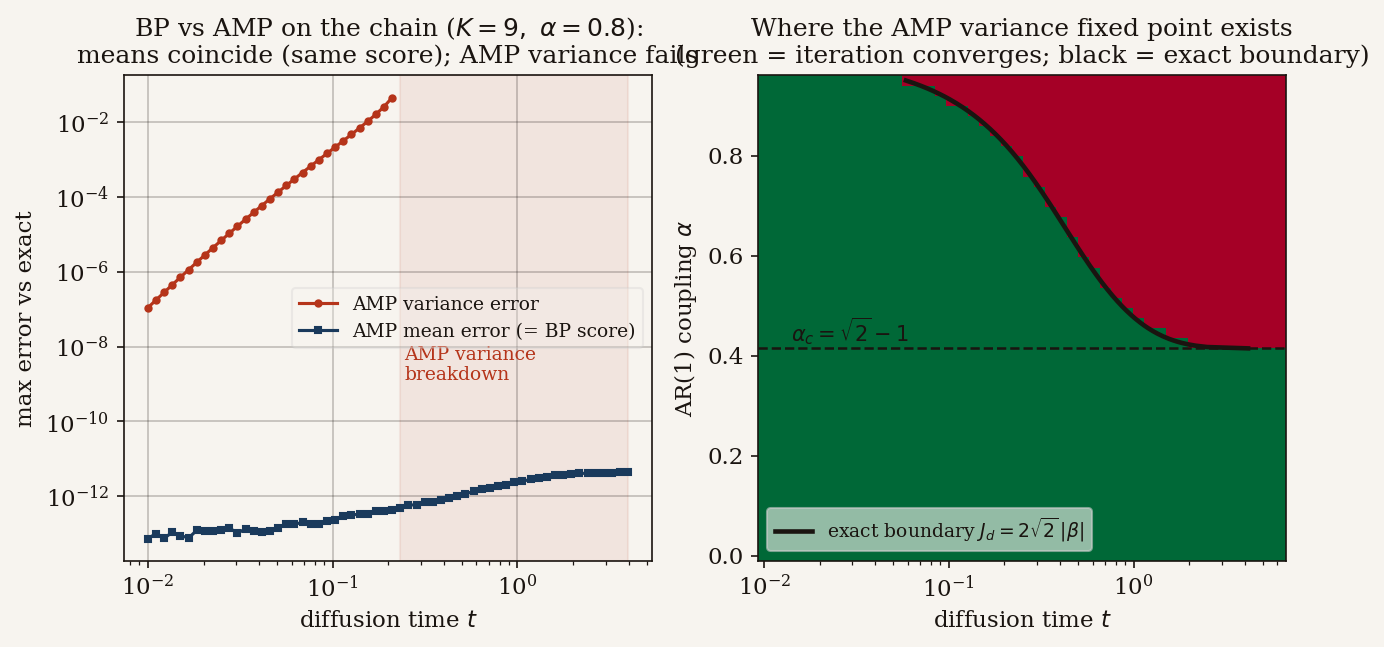
\includegraphics[width=\linewidth]{figures/fig_bp_vs_amp.png}
\caption{\textbf{BP vs.\ AMP on a finite chain ($K=9$, $\alpha=0.8$).} Left:
the AMP \emph{mean} error (navy, $\sim10^{-12}$, flat in $t$) --- the score is
closure-independent (Theorem~\ref{thm:same-score}); the AMP \emph{variance}
error (red) grows with $t$ until the closure stops converging (shaded).
Right: where the AMP variance fixed point exists in the $(\alpha,t)$ plane;
green$\,=\,$the self-consistent iteration converges, and the black curve is
the \emph{exact} boundary $t_c(\alpha)$ of \eqref{eq:tc} with the horizontal
dashed line at $\alpha_c=\sqrt2-1$. Theory and iteration agree at all 180
scanned points.}
\label{fig:bpamp}
\end{figure}

\begin{intuition}[: the precise content of ``a CLT on two points'']
J.~Garnier-Brun's remark --- that AMP's Gaussian-message assumption is a
central limit statement that ``on two data points is usually not right'' ---
is here made exact. On the chain, dropping the cavity exclusion replaces
$\beta^2$ by $2\beta^2$ in the fixed-point equation; the discriminant moves
from $\Jd^2-4\beta^2$ (never negative) to $\Jd^2-8\beta^2$ (negative beyond
\eqref{eq:tc}). At weak coupling the sin is venial
(\eqref{eq:weak}: a fourth-order overestimate); at strong coupling it is
mortal (no fixed point at all). Meanwhile on a dense problem the same closure
is excellent --- the audit's dense gate ($N=600$ random SPD precision) shows
AMP variance error $1.7\times10^{-3}$ against mean field's $4\times10^{-2}$.
AMP is not wrong; it is \emph{built for a different graph}.
\end{intuition}

\begin{auditbox}[: every claim of this section, measured]
(i) AMP mean $=$ exact mean to $4.3\times10^{-12}$ and AMP score $=$ BP score
to $1.7\times10^{-12}$ over $36$ chain configurations
(Theorem~\ref{thm:same-score}). (ii) $V_{\textsc{amp}}$ from
\eqref{eq:amp-fixed} matches the converged self-consistent iteration at the
centre of a $K=400$ chain to $2.5\times10^{-12}$ ($12$ configurations).
(iii) The existence condition \eqref{eq:amp-exists} predicts the convergence
/ non-convergence of the iteration at all $180$ points of an $(\alpha,t)$
scan. (iv) $t_c$ from \eqref{eq:tc} matches the bisected flip point of the
iteration to $6.6\times10^{-6}$ relative. (v) Below $\alpha_c$ the iteration
converges even at $t=50$. (vi) The weak-coupling ratio
$(V_{\textsc{amp}}-V_{\mathrm{exact}})/(2\beta^4/\Jd^5)\to1$ within
$0.4\%$ at the smallest couplings tested.
\end{auditbox}

% =============================================================================
\section{Experiment A: local messages versus full sweeps}\label{sec:expA}
% =============================================================================

How much does a frame's score depend on \emph{distant} frames? This was one of
the two experimental questions posed in discussion, and the bulk analysis of
\S\ref{sec:bulk} lets us answer it exactly rather than only empirically.

\subsection{The local estimator and the exact error measure}

Define the \emph{local estimator of radius $r$} as the posterior mean of
$a_k$ given only the observations within distance $r$,
\[
  m^{(r)}_k:=\E\big[a_k\,\big|\,x_{k-r},\dots,x_{k+r}\big],
\]
the rest of the chain marginalised out, and the corresponding score via
Tweedie. Two structural facts make this a \emph{clean} experiment:
\begin{itemize}[leftmargin=1.6em, itemsep=1pt]
\item \textbf{Exactness on the window.} Any contiguous block of a stationary
\textsc{ar}(1) chain is itself a stationary \textsc{ar}(1) chain, so
$m^{(r)}_k$ is computed \emph{exactly} on the windowed sub-chain --- the only
approximation in play is the truncation of range. At $r\ge K-1$ the window is
the whole chain and the estimator is exact (audited: $3.6\times10^{-15}$).
\item \textbf{A deterministic error.} Both $m_k$ and $m^{(r)}_k$ are linear
in $x$, so their difference is $e\T x$ for a computable row vector $e$, and
the root-mean-square error over the data distribution $x\sim P_t=\N(0,\Sig_t)$
is the closed-form number
\[
  \mathrm{RMS}_r(k)=\sqrt{e\T\Sig_t\,e}
\]
--- no sampling, no seed, nothing to tune. (Code:
\texttt{local\_bp.rms\_truncation\_error}.)
\end{itemize}

\subsection{The locality law}

\begin{theorem}[Locality error decays exactly as $q^{\,r}$]\label{thm:locality}
In the bulk, $\log\mathrm{RMS}_r(k)$ decreases linearly in $r$ with slope
$\log q$, where $q=q(\alpha,t)$ is the posterior correlation decay rate of
Theorem~\ref{thm:bulk-cov}. Equivalently: truncating the message range at $r$
costs a factor $q$ per discarded frame.
\end{theorem}

\begin{derivation}[\ref*{thm:locality}: why the rate must be $q$ --- and how it
is verified]
The error of the radius-$r$ estimator is the influence on
$\E[a_k\given\cdot\,]$ of the evidence beyond the window. In the Gaussian
chain, the influence of evidence at frame $k\pm d$ on the posterior mean at
$k$ is proportional to the posterior covariance $(J^{-1})_{k,k\pm d}$, which
by Theorem~\ref{thm:bulk-cov} decays as $q^{\,d}$. The leading discarded
contribution sits at distance $r+1$, so the error inherits the geometric rate
$q$ per unit radius (the prefactor sums the geometric tail and the data
covariance). Rather than chase the prefactor analytically, we verify the
\emph{rate}: the audit fits the slope of $\log\mathrm{RMS}_r$ over
$r=2,\dots,13$ at the centre of a $K=121$ chain and finds it equal to
$\log q$ within $0.2\%$ at $t\in\{0.1,0.5,2.0\}$ ($\alpha=0.8$).
\end{derivation}

\begin{figure}[h]\centering
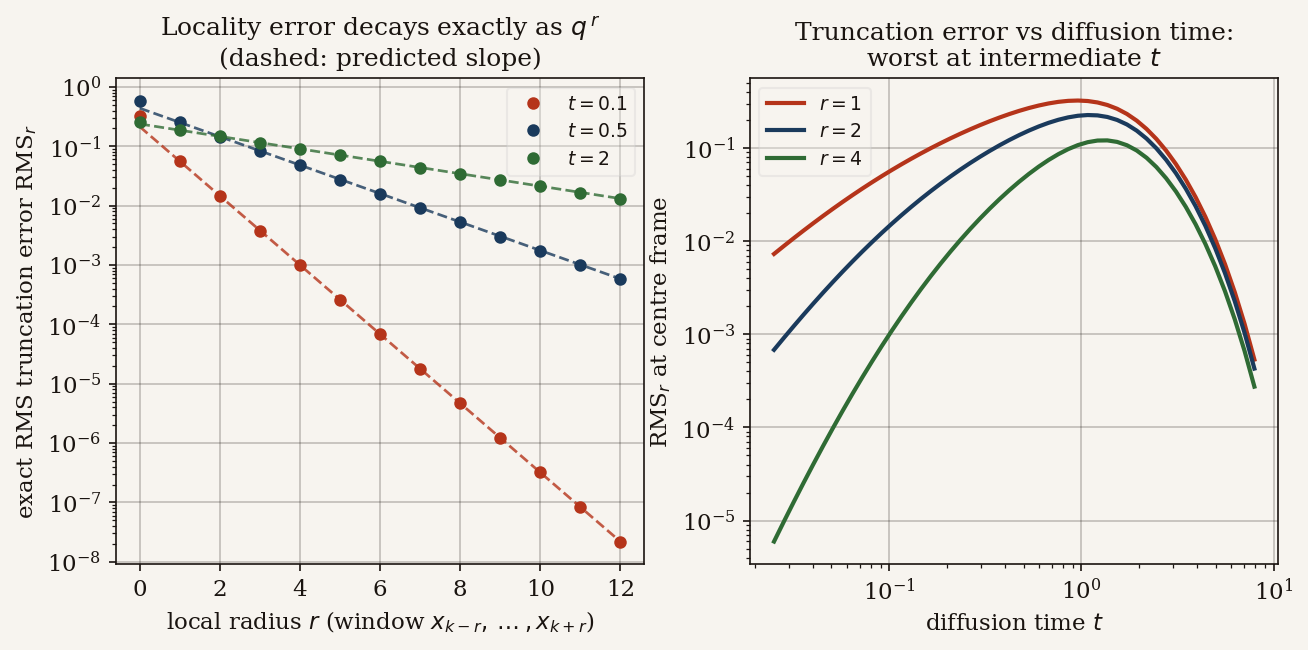
\includegraphics[width=\linewidth]{figures/fig_local_vs_full.png}
\caption{\textbf{Locality of the joint score.} Left: exact RMS truncation
error of the radius-$r$ estimator (dots) at three diffusion times; the dashed
lines have the \emph{predicted} slopes $q(\alpha,t)^{\,r}$ from
\eqref{eq:bulk-cov} --- no fitting. Right: the same error at fixed radius as
a function of $t$: it vanishes at $t\to0$ (each frame pinned by its own
observation: $q\to0$) and at $t\to\infty$ (the \emph{score} decouples as
$Q_t\to I$, and the signal itself dies), and peaks at intermediate $t$.}
\label{fig:local}
\end{figure}

\begin{intuition}[: the answer to ``local messages vs full sweeps'']
Strictly-neighbour messages ($r=1$) are exact at $t=0$, excellent at small
$t$, and wrong by a factor governed by $q^{\,2}$ relative reach at
intermediate $t$; the full sweeps are exact always. The cost of locality is
not a constant --- it is a \emph{rate}, $q(\alpha,t)$ per frame of range, and
that rate is largest precisely in the mid-diffusion regime where generative
sampling spends its critical steps (cf.\ the tilted-measure crossover of
\S\ref{sec:noisy}). In the Gaussian case the local approximation is thus
completely \emph{quantified}: choose the radius $r$ as
$r\gtrsim\xi\log(1/\varepsilon)$ with $\xi=1/\log(1/q)$ to guarantee relative
error $\varepsilon$.
\end{intuition}

% =============================================================================
\section{Experiment B: lifecycle of the precision matrix}\label{sec:expB}
% =============================================================================

The score \eqref{eq:score-matrix} is entirely controlled by
$\Qt=\Sig_t^{-1}$, and a zero of $\Qt$ is a conditional independence of
$P_t$. This experiment tracks how the sparsity pattern of $\Qt$ is born,
lives and dies along diffusion time --- the question raised in the project
notebook (``the zeros should progressively fill up\dots\ then identity
again'').

\subsection{Three equivalent forms of $\Qt$}

\begin{theorem}[Three forms]\label{thm:three-forms}
For all $t\ge0$, with $\gamma_t:=e^{-2t}/\Dt$ (the SNR) and
$c_t:=e^{2t}-1$:
\begin{align}
  \Qt&=\tfrac1\Dt\big(I+\gamma_t\,\Sig_0\big)^{-1}
  &&\text{(SNR form)},\label{eq:Qt-snr}\\
  \Qt&=U\,\diag\!\Big(\frac{1}{e^{-2t}\omega_i+\Dt}\Big)\,U\T,
  \qquad \Sig_0=U\diag(\omega_i)U\T
  &&\text{(spectral form)},\label{eq:Qt-spec}\\
  \Qt&=e^{2t}\,Q_0\big(I+c_tQ_0\big)^{-1}
     =e^{2t}\sum_{m\ge0}(-c_t)^m\,Q_0^{\,m+1}
  &&\text{(resolvent form)}.\label{eq:Qt-res}
\end{align}
\end{theorem}

\begin{derivation}[\ref*{thm:three-forms}]
\textbf{SNR.} Factor $\Dt$ out of \eqref{eq:Sigt} and invert.
\textbf{Spectral.} $I$ commutes with everything:
$\Sig_t=U\diag(e^{-2t}\omega_i+\Dt)U\T$, and inverting a diagonal is
entry-wise. \textbf{Resolvent.} Multiply \eqref{eq:Sigt} on the left by
$Q_0$: $Q_0\Sig_t=e^{-2t}(I+c_tQ_0)$ using $\Dt e^{2t}=c_t$; invert both
sides. The Neumann series converges for $\|c_tQ_0\|<1$, the small-$t$ /
high-SNR regime. \qed
\end{derivation}

\begin{intuition}[: locality is a basis-dependent statement]
The spectral form says the eigenvectors of $\Sig_t$ and $\Qt$ are those of
$\Sig_0$ \emph{for every $t$} --- only the eigenvalues flow,
$\omega_i\mapsto e^{-2t}\omega_i+\Dt\to1$. In the $\Sig_0$-eigenbasis
(near-Fourier modes, since $\Sig_0$ is symmetric Toeplitz) the denoising
problem decouples into $K$ scalar problems at all times: maximal locality. In
the \emph{frame} basis --- the operationally meaningful one for video ---
$\Qt$ is tridiagonal only at $t=0$. Both statements describe the same matrix;
sparsity is a property of a matrix \emph{in a basis}.
\end{intuition}

\begin{figure}[h]\centering
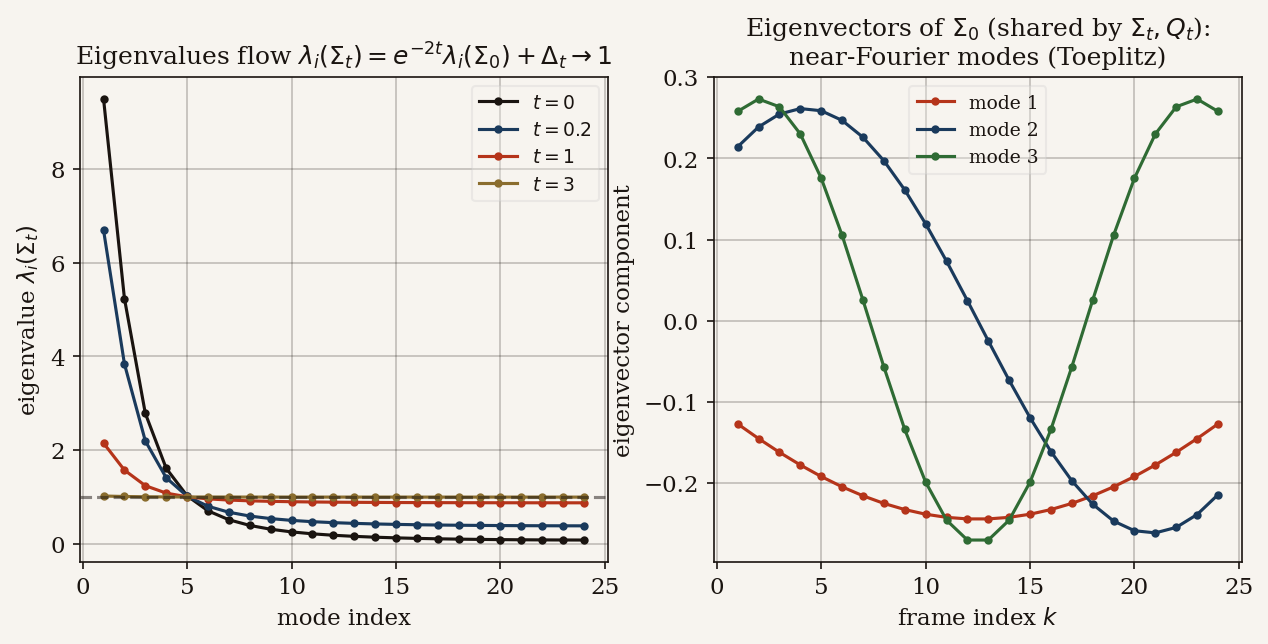
\includegraphics[width=\linewidth]{figures/fig_spectral.png}
\caption{\textbf{Spectral lifecycle.} Left: eigenvalues of $\Sig_t$ flow as
$e^{-2t}\omega_i+\Dt$, all toward $1$. Right: the shared eigenvectors of
$\Sig_0$ (hence of $\Sig_t,\Qt$ at every $t$) are near-Fourier modes.}
\label{fig:spectral}
\end{figure}

\subsection{The band-fill law (corrected)}

\begin{figure}[h]\centering
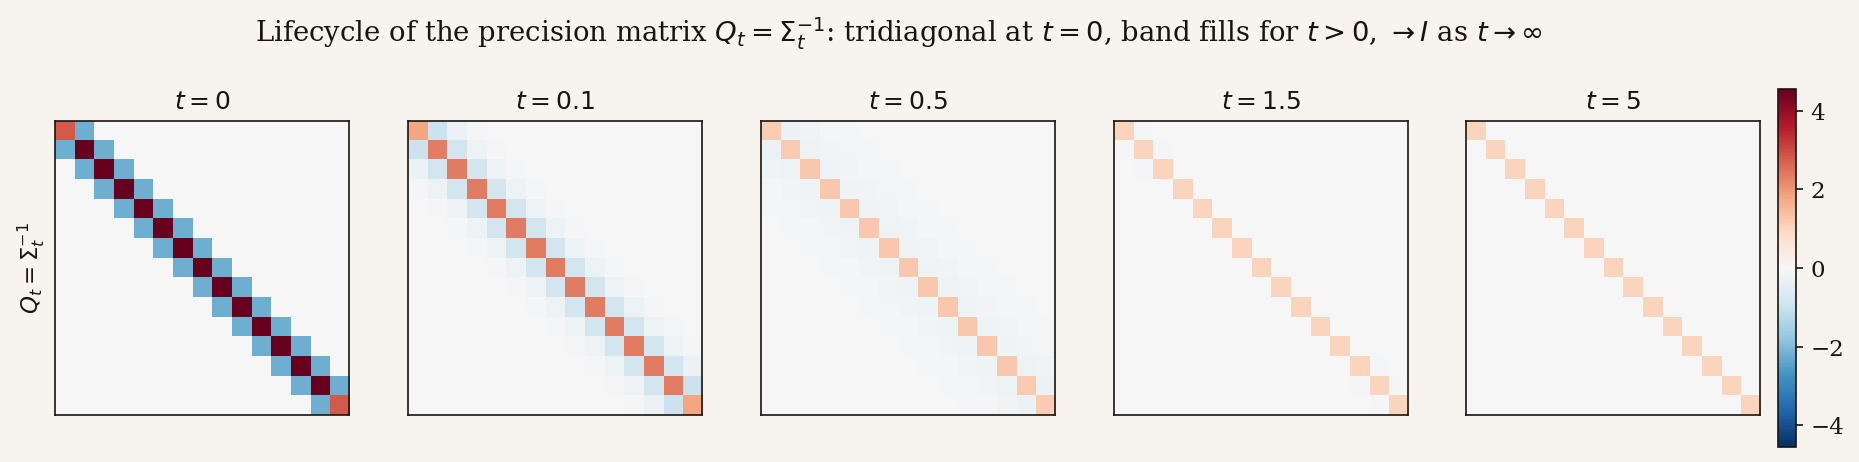
\includegraphics[width=\linewidth]{figures/fig_precision_lifecycle.png}
\caption{\textbf{Lifecycle of $\Qt$ in the frame basis} ($K=15$,
$\alpha=0.8$). Tridiagonal at $t=0$ (Markov); the band fills for $t>0$
(dense); the magnitude collapses and $\Qt\to I$ as $t\to\infty$ (isotropic
noise wins).}
\label{fig:lifecycle}
\end{figure}

\begin{theorem}[Band-fill leading order --- no factorial]\label{thm:bandfill}
For small $t$ and frame distance $d\ge1$,
\begin{equation}\label{eq:bandfill}
  \boxed{\ (\Qt)_{i,i+d}=(-1)^{d-1}\,(2t)^{d-1}\,(Q_0^{\,d})_{i,i+d}
  \;+\;O(t^{d})\ }
\end{equation}
\end{theorem}

\begin{derivation}[\ref*{thm:bandfill}: Neumann series of the resolvent]
In \eqref{eq:Qt-res}, substitute $c_t=2t+2t^2+O(t^3)$ and
$e^{2t}=1+O(t)$:
\[
  \Qt=(1+O(t))\big[\,Q_0-c_tQ_0^2+c_t^2Q_0^3-\cdots\big].
\]
$Q_0$ is tridiagonal, so $Q_0^{\,m}$ has bandwidth $m$: the entry at distance
$d$ receives its first contribution from the term $m=d$, which enters the
series with prefactor $(-c_t)^{d-1}=(-1)^{d-1}(2t)^{d-1}(1+O(t))$. All higher
terms are $O(t^{d})$. \qed
\end{derivation}

\begin{remark}[Correction to a previously circulated formula]\label{rmk:corr}
An earlier internal note (\texttt{precision\_lifecycle\_summary.pdf},
eq.~(12)) printed \eqref{eq:bandfill} with an extraneous $1/(d-1)!$ factor.
That factor does not follow from the resolvent expansion --- the leading
distance-$d$ term is the \emph{single} contribution $m=d$, with no
combinatorial sum behind it --- and the audit rejects it: the no-factorial
coefficient matches the measured $(\Qt)_{i,i+d}/t^{d-1}$ to better than
$0.9\%$ for every $d\in\{1,\dots,5\}$ ($\alpha=0.9$, $K=25$), while the
factorial version fails by $86\%$ at $d=3$, $290\%$ at $d=4$, $800\%$ at
$d=5$. (Empirical \emph{slope} fits cannot distinguish the two --- the slopes
$d-1$ are prefactor-blind --- which is how the error survived until the
coefficient itself was audited. A useful lesson about checking
coefficients, not just exponents.)
\end{remark}

\begin{figure}[h]\centering
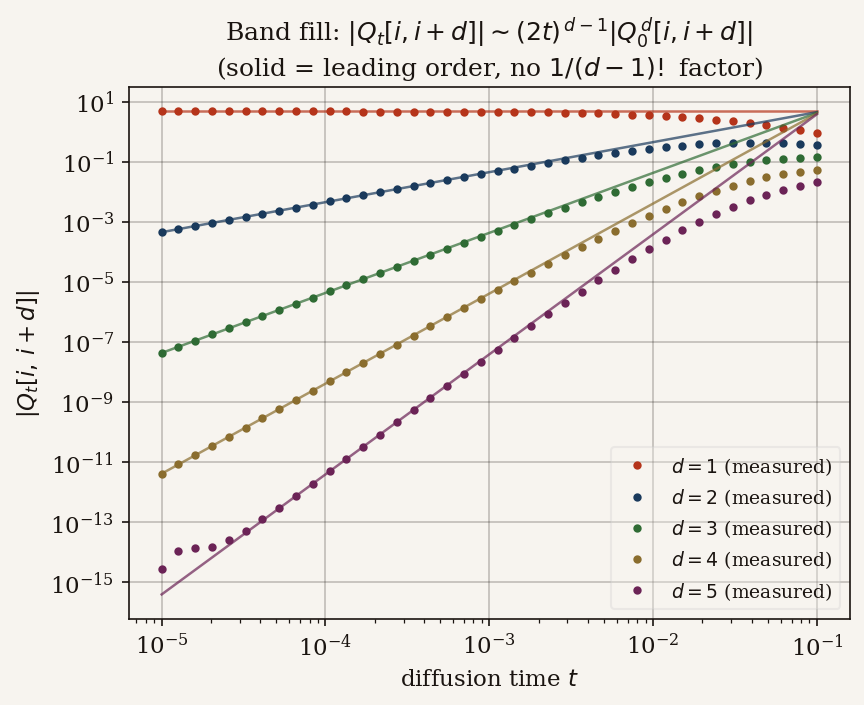
\includegraphics[width=0.74\linewidth]{figures/fig_band_fill.png}
\caption{\textbf{Band fill, log--log.} Measured $|(\Qt)_{i,i+d}|$ (dots)
against the leading order \eqref{eq:bandfill} (solid; no factorial). Slopes
$d-1=0,\dots,4$; the agreement at small $t$ is at the percent level for every
$d$.}
\label{fig:bandfill}
\end{figure}

\subsection{Return to the identity, and one number for the whole lifecycle}

\begin{proposition}[Large-$t$ return]\label{prop:larget}
As $t\to\infty$, writing $\Sig_t=I+e^{-2t}(\Sig_0-I)$,
\[
  \Qt=I-e^{-2t}(\Sig_0-I)+e^{-4t}(\Sig_0-I)^2+O(e^{-6t}),
\]
so $\|\Qt-I\|_F\simeq e^{-2t}\|\Sig_0-I\|_F$: every correlation dies at the
universal rate $e^{-2t}$ and the score collapses to the isotropic $-x$.
(Audited at $t\in\{3,6,10\}$.)
\end{proposition}

\begin{figure}[h]\centering
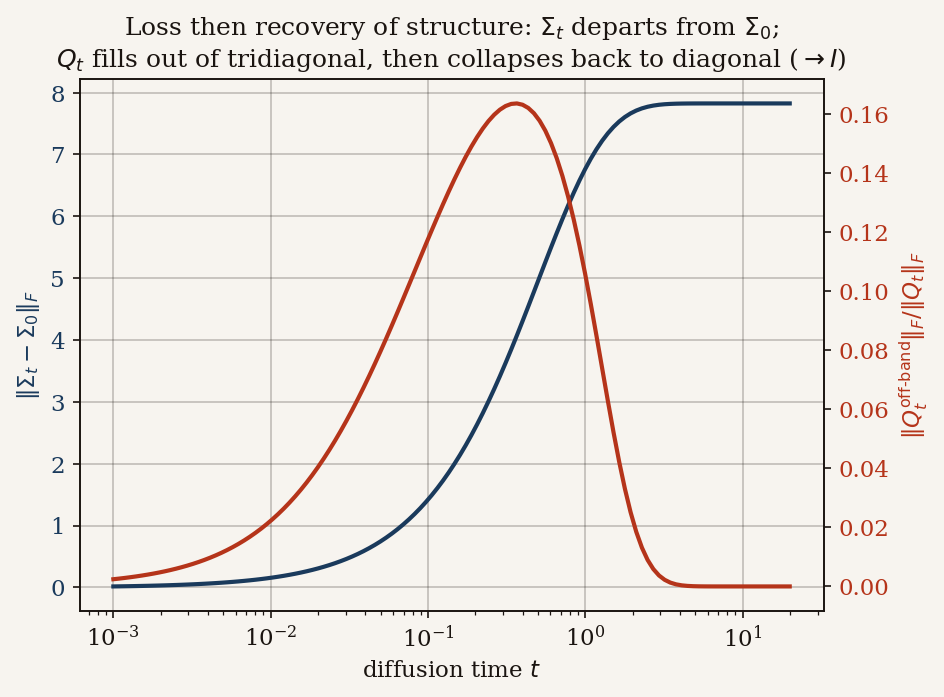
\includegraphics[width=0.74\linewidth]{figures/fig_tridiag_loss.png}
\caption{\textbf{Loss then recovery of structure, in one curve each.}
$\|\Sig_t-\Sig_0\|_F$ (navy) grows monotonically as the covariance is driven
to $I$; the off-tridiagonal Frobenius mass of $\Qt$ (red) rises from zero,
peaks at intermediate $t$, and decays back to zero --- the band fills, then
empties.}
\label{fig:tridiagloss}
\end{figure}

\begin{intuition}[: Experiments A and B are the same fact, twice]
The lifecycle of $\Qt$ (Exp.~B) and the locality error (Exp.~A) are two views
of one object: how far apart frames talk to each other through the score. At
$t=0$ the conversation is nearest-neighbour ($\Qt$ tridiagonal; $q=0$); at
intermediate $t$ it has range $\xi=1/\log(1/q)$ (band filled; locality error
maximal); at $t\to\infty$ it ceases ($\Qt\to I$; everything decouples). The
bulk parameter $q(\alpha,t)$ of \S\ref{sec:bulk} is the single dial behind
both pictures.
\end{intuition}

% =============================================================================
\section{Summary of established results, and what comes next}\label{sec:summary}
% =============================================================================

\subsection{What is established}

Every row below is closed-form, derived in this note, and verified by the
named audit section (Appendix~\ref{app:audit}).

\begin{center}\small
\begin{tabular}{@{}p{0.62\textwidth}ll@{}}
\toprule
Result & Where & Audit\\
\midrule
Clean precision $Q_0$ tridiagonal, entries explicit & Prop.~\ref{prop:Q0} & \S1\\
$\Sig_t=e^{-2t}\Sig_0+\Dt I$; score $S=-\Qt x$ & Prop.~\ref{prop:Sigt} & \S2\\
Tweedie: $S_k=(e^{-t}\E[a_k|x]-x_k)/\Dt$, two routes agree & Th.~\ref{thm:tweedie} & \S6\\
$K=2$ fully explicit; coupling $r=\alpha e^{-2t}$ & \S\ref{sec:K2} & \S10\\
Posterior $J=(e^{-2t}/\Dt)I+Q_0$, $h=(e^{-t}/\Dt)x$ & Prop.~\ref{prop:posteriorJ} & \S5,6\\
Factor graph is a tree; BP exact, $O(K)$; Convention A & Props.~\ref{prop:tree},\ref{prop:convA} & \S5\\
All messages Gaussian by algebraic closure (no CLT) & Th.~\ref{thm:closure} & \S5\\
BP $=$ Kalman filter $+$ RTS smoother; machine precision & \S\ref{sec:bpK} & \S5\\
Bulk: $\lambda^\ast=(\Jd{+}\sqrt{\Jd^2{-}4\beta^2})/2$ exists always & Th.~\ref{thm:bp-bulk} & \S11\\
Bulk variance $1/\sqrt{\Jd^2-4\beta^2}$; covariance $q^{\,d}V$ & Ths.~\ref{thm:bp-bulk},\ref{thm:bulk-cov} & \S11\\
Same mean $\Rightarrow$ BP, AMP, MF give the \emph{same score} & Th.~\ref{thm:same-score} & \S7\\
AMP variance $V=(\Jd{-}\sqrt{\Jd^2{-}8\beta^2})/4\beta^2$; exists iff $\Jd\ge2\sqrt2|\beta|$ & Th.~\ref{thm:amp-bulk} & \S8,11\\
Exact breakdown time $t_c(\alpha)$; critical coupling $\alpha_c=\sqrt2-1$ & Th.~\ref{thm:amp-bulk} & \S11\\
Weak coupling: $V_{\textsc{amp}}-V_{\mathrm{ex}}=2\beta^4/\Jd^5+\dots$ & Th.~\ref{thm:weak} & \S11\\
Locality error decays exactly as $q^{\,r}$ & Th.~\ref{thm:locality} & \S9,11\\
Band fill $(\Qt)_{i,i+d}=(-1)^{d-1}(2t)^{d-1}(Q_0^d)_{i,i+d}+O(t^d)$, \emph{no} $1/(d{-}1)!$ & Th.~\ref{thm:bandfill} & \S3\\
Spectral preservation; large-$t$ return $\Qt\to I$ at rate $e^{-2t}$ & Th.~\ref{thm:three-forms}, Prop.~\ref{prop:larget} & \S2,4\\
\bottomrule
\end{tabular}
\end{center}

\subsection{The structural moral}

The posterior of a Markov sequence under frame-wise noise \emph{is} a
caterpillar tree, and the joint score \emph{is} a smoothing problem on that
tree. An architecture that hard-codes this graph gets exactness and $O(K)$
cost for free in the Gaussian case --- and retains the correct \emph{structure}
(the recursions \eqref{eq:fwd-rec}--\eqref{eq:bwd-rec}) for any Markov prior,
Gaussian or not; only the message \emph{parametrisation} changes. This is the
same shift that took vision from generic MLPs to convolutions: encode what is
known about the data --- here, its internal Markov time --- into the
computation, instead of spending capacity rediscovering it. AMP is the wrong
inductive bias for this graph, and \S\ref{sec:amp} now says so with an exact
phase boundary rather than a heuristic.

\subsection{Research directions}

\begin{enumerate}[leftmargin=1.6em, itemsep=2pt]
\item \textbf{Non-Gaussian prior (Laplace \textsc{ar}(1)).} Gaussian closure
is the only Gaussian-specific ingredient of the whole construction. With
Laplace innovations the recursions \eqref{eq:fwd-rec}--\eqref{eq:bwd-rec}
survive but messages become genuine functions; preliminary work shows the
\emph{boundary} message retains a clean closed form while interior messages do
not --- the natural next document mirrors this one with messages tracked
numerically on a grid, the audit discipline unchanged.
\item \textbf{The propagator question.} In the stationary bulk, $\Qt$ is
(asymptotically) Toeplitz, so consecutive rows of the score operator are
shifts of one another --- the formal skeleton of the propagator hypothesis
$S_{k+1}\approx P_t\,S_k$. The bulk analysis of \S\ref{sec:bulk} (the
$q$-geometric structure of $J^{-1}$, hence of $\Qt$ by the same
transfer-matrix argument) is the right starting point for making $P_t$
explicit and quantifying its boundary corrections.
\item \textbf{Local score architectures.} Theorem~\ref{thm:locality} gives a
principled radius: $r\approx\xi\log(1/\varepsilon)$ with
$\xi=1/\log(1/q(\alpha,t))$ --- a noise-level-dependent receptive field. It
would be instructive to test whether trained video-score networks develop
receptive fields tracking $\xi(t)$.
\item \textbf{Beyond scalar frames.} For $a_k\in\R^d$ with linear dynamics,
every formula survives with $\alpha\to A$ (a matrix) and Kalman algebra;
the bulk analysis becomes a matrix quadratic --- worth writing once a concrete
$d>1$ toy (e.g.\ the rotating frame) is fixed.
\end{enumerate}

% =============================================================================
\section{Reproducibility}\label{sec:repro}
% =============================================================================

Everything in this note is reproducible from the repository
\href{https://github.com/GioviManto/gaussian-bp-diffusion}{\texttt{GioviManto/gaussian-bp-diffusion}}:

\begin{itemize}[leftmargin=1.6em, itemsep=1pt]
\item \texttt{code/ar1\_utils.py} --- model: $\Sig_0$, $Q_0$, $\Sig_t$,
$\Qt$ (direct and spectral), exact score (matrix and Tweedie), posterior.
\item \texttt{code/bp\_score.py} --- Convention-A BP: forward / backward
sweeps, combination, BP score.
\item \texttt{code/chain\_formulas.py} --- every closed form of
\S\ref{sec:bulk}--\ref{sec:amp}: $\Jd,\beta$, $\lambda^\ast$,
$V_{\mathrm{exact}}$, $q$, bulk covariance, $V_{\textsc{amp}}$, existence,
$t_c$, $\alpha_c$, weak-coupling error; and the $K=2$ forms of \S\ref{sec:K2}.
\item \texttt{code/amp.py} --- the three marginal schemes (mean field,
AMP/TAP, exact) on arbitrary $(J,h)$; honest breakdown reporting.
\item \texttt{code/local\_bp.py} --- radius-$r$ local estimator and the exact
RMS truncation error.
\item \texttt{code/experiments.py} --- all figures.
\item \texttt{code/numerical\_audit.py} --- the gate: \textbf{72 checks},
all passing.
\item \texttt{01\_model\_and\_score.ipynb},
\texttt{02\_belief\_propagation.ipynb},
\texttt{03\_amp\_and\_experiments.ipynb} --- executed companions mirroring
\S\ref{sec:setup}--\ref{sec:K2}, \S\ref{sec:posterior}--\ref{sec:bpK}, and
\S\ref{sec:bulk}--\ref{sec:expB} respectively.
\end{itemize}

\noindent To reproduce from scratch:
\begin{quote}\small\ttfamily
python3 -m venv .venv \&\& source .venv/bin/activate\\
pip install numpy matplotlib jupyter nbclient nbformat\\
python code/numerical\_audit.py\hspace{2.2em}\#\ ->\ PASSED 72 / 72\\
python code/experiments.py\hspace{4.05em}\#\ ->\ figures/*.png\\
python build\_companions.py\hspace{3.6em}\#\ ->\ the three executed notebooks\\
tectonic main.tex\hspace{7.45em}\#\ ->\ main.pdf
\end{quote}

% =============================================================================
\appendix
\section{The numerical audit, section by section}\label{app:audit}
% =============================================================================

The audit philosophy: \emph{a statement enters the text only if an independent
check passes}. Independent means: the closed form is compared against a
different computational route (brute-force inversion, spectral identity,
bisection of an iteration, a fitted slope), never against itself. The 72
checks group as follows; worst errors are over all configurations in each
group.

\begin{center}\small
\begin{tabular}{@{}cp{0.52\textwidth}ccc@{}}
\toprule
\S & contents & checks & worst error & tolerance\\
\midrule
1 & $Q_0=\Sig_0^{-1}$ exactly tridiagonal (12 configs) & 24 & $1.8\times10^{-14}$ & $10^{-12}$/exact\\
2 & $\Sig_t\Qt=I$; spectral form; $U$ diagonalises $\Sig_0$ & 15 & $2.2\times10^{-14}$ & $10^{-10}$\\
3 & band-fill coefficient, $d=1..5$ (no factorial) & 5 & $9.0\times10^{-3}$ & $5\times10^{-2}$\\
4 & large-$t$ return $\|\Qt-I\|_F\sim e^{-2t}$ & 3 & $2.1\times10^{-2}$ & struct.\\
5 & BP vs matrix: mean / variance / score (80 configs) & 3 & $1.2\times10^{-14}$ & $10^{-10}$\\
6 & Tweedie route $=$ matrix route & 1 & $2.7\times10^{-15}$ & $10^{-12}$\\
7 & AMP mean $=$ exact; AMP score $=$ BP score (36 configs) & 2 & $4.3\times10^{-12}$ & $10^{-9}$\\
8 & AMP variance: dense-graph accuracy; chain breakdown & 4 & $1.7\times10^{-3}$ & $5\times10^{-2}$\\
9 & local BP: $r{=}K{-}1$ exact; error monotone in $r$ & 2 & $3.6\times10^{-15}$ & $10^{-9}$\\
10 & $K=2$ closed forms: $\Sig_t$, $\Qt$, score & 3 & $1.8\times10^{-15}$ & $10^{-12}$\\
11 & bulk closed forms: $V_{\mathrm{exact}}$, recombination and existence,
     $V_{\textsc{amp}}$, boundary scan, $q^{\,d}$ covariance, weak-coupling
     ratio, locality slope, $t_c$, $\alpha_c$ & 10 & $3.4\times10^{-3}$ & varies\\
\bottomrule
\end{tabular}
\end{center}

\noindent Run \texttt{python code/numerical\_audit.py} to regenerate the full
72-line report; each line names the claim, the measured error, and the
tolerance.

\bibliographystyle{plainnat}
\bibliography{references}

\end{document}
